% ---------------------------------------------------
% Trabajo Fin de Grado:
% Author: Álvaro Fontenla León <alu0101437989@ull.edu.es>
% Author: F. de Sande fsande@ull.es
%
% ----------------------------------------------------
% 
\documentclass[english,a4paper,12pt,oneside]{extreport}
\usepackage{listingsutf8}
\usepackage{listings}
\usepackage[scale=0.82]{FiraMono}
\usepackage[T1]{fontenc}
%\documentclass[a4paper, twoside, 12pt]{book}
\usepackage[a4paper]{geometry}
\usepackage[spanish, main=english]{babel}
\usepackage[utf8]{inputenc}
\usepackage{lmodern,textcomp}  % For € symbol
\usepackage{pdflscape}
\usepackage{amsmath}
\usepackage{array}
\newcolumntype{C}[1]{>{\centering\arraybackslash}m{#1}}
\usepackage{makecell}
\usepackage{multirow}
%%%%%%%%%%%%%%%%%%%%%%%%%%%%%%%%%%%%%%%%%%%%%%%%%%%%%%%%%%%%%%%%%%%%%%%%%%%%%%%%%%%%%%%%%%%%
% Next 3+3 lines select PDF or PS output (comment as apropriate)
% To switch from PDF and PS comment/uncomment here and change Makefile
\usepackage[pdftex]{xcolor}
\usepackage[pdftex]{graphicx}
\graphicspath{{images/}}
%\usepackage[dvips]{color}
%\usepackage[dvips]{graphicx}
\usepackage{epsfig}
%\graphicspath{{images/eps/}}
\usepackage{floatrow}
\usepackage{tabu}

%%%%%%%%%%%%%%%%%%%%%%%%%%%%%%%%%%%%%%%%%%%%%%%%%%%%%%%%%%%%%%%%%%%%%%%%%%%%%%%%%%%%%%%%%%%%
\usepackage{algorithmic}
%\usepackage[pdftex=true,colorlinks=false,urlcolor=blue,plainpages=false,pagebackref=true,citecolor=red]{hyperref} %hiperenlaces y backcites
\usepackage[colorlinks=true,urlcolor=blue,plainpages=false,pagebackref=true,citecolor=black]{hyperref} %hiperenlaces y backcites
\hypersetup{breaklinks=true}
% Redefinir el comando \url para cambiar el tamaño del texto de los enlaces
% \let\oldurl\url
% \renewcommand{\url}[1]{{\scriptsize{\oldurl{#1}}}}

\usepackage{url}
\usepackage{subcaption}
%%%%%%%%%%%%%%%%%%%%%%%%%%%%%%%%%%%%%%%%%%%%%%%%%%%%%%%%%%%%%%%%%%%%%%%%%%%%%%%%%%%%%%%%%%%
% Comandos para escribir "siempre igual"
\newcommand{\TitleTopic}{\texttt{Título}}


%%% Traducimos el pseudocodigo
\renewcommand{\algorithmicwhile}{\textbf{mientras}}
\renewcommand{\algorithmicend}{\textbf{fin}}
\renewcommand{\algorithmicdo}{\textbf{hacer}}
\renewcommand{\algorithmicif}{\textbf{si}}
\renewcommand{\algorithmicthen}{\textbf{entonces}}
\renewcommand{\algorithmicrepeat}{\textbf{repetir}}
\renewcommand{\algorithmicuntil}{\textbf{hasta que}}
\renewcommand{\algorithmicelse}{\textbf{en otro caso}}
\renewcommand{\algorithmicfor}{\textbf{para}}

%%%%%%%%%%%%%%%%% Se crea un entorno para listar código fuente %%%%%%%%%%%%%%%
\newenvironment{sourcecode}
{\begin{list}{}{\setlength{\leftmargin}{1em}}\item\scriptsize\bfseries}
{\end{list}}

\newenvironment{littlesourcecode}
{\begin{list}{}{\setlength{\leftmargin}{1em}}\item\tiny\bfseries}
{\end{list}}

\newenvironment{summary}
{\par\noindent\begin{center}\textbf{Abstract}\end{center}\begin{itshape}\par\noindent}
{\end{itshape}}

\newenvironment{keywords}
{\begin{list}{}{\setlength{\leftmargin}{1em}}\item[\hskip\labelsep \bfseries Keywords:]}
{\end{list}}

\newenvironment{palabrasClave}
{\begin{list}{}{\setlength{\leftmargin}{1em}}\item[\hskip\labelsep \bfseries Palabras clave:]}
{\end{list}}

%%%%%%%%%%%%%%%%%%%%%%%%%%%%%%%%%%%%%%%%%%%%%%%%%%%%%%%%%%%%%%%%%%%%%%%%%%%%%%%
\definecolor{marron}       {rgb}{0.496, 0.203, 0.152}
\definecolor{verde-claro}  {rgb}{0.625, 0.734, 0.199}
\definecolor{oscuro}       {rgb}{0.187, 0.141, 0.285}
\definecolor{gris}     	   {rgb}{0.500, 0.500, 0.500}
\definecolor{bgd-listings} {rgb}{0.999, 0.999, 0.900}
\definecolor{gray97}{gray}{.97}
\definecolor{gray75}{gray}{.75}
\definecolor{gray45}{gray}{.45}
\definecolor{gray}{gray}{.45}
\definecolor{Brown}{cmyk}{0,0.81,1,0.60}
\definecolor{OliveGreen}{cmyk}{0.64,0,0.95,0.40}
\definecolor{CadetBlue}{cmyk}{0.62,0.57,0.23,0}
\definecolor{lightlightgray}{gray}{0.9}
%%%%%%%%%%%%%%%%%%%%%%%%%%%%%%%%%%%%%%%%%%%%%%%%%%%%%%%%%%%%%%%%%%%%%%%%%%%%%%%%%%%%%%%%%%%
%Evitar partir palabras al final de la línea
\hyphenpenalty=10000
\tolerance=1000
%%%%%%%%%%%%%%%%%%%%%%%%%%%%%%%%%%%%%%%%%%%%%%%%%%%%%%%%%%%%%%%%%%%%%%%%%%%%%%%%%%%%%%%%%%%%
% Para listados de código
\usepackage{listings}
% \lstloadlanguages{C,C++}
%\lstloadlanguages{python,C}

% Definiendo colores para los listados de código fuente - Univ. Deusto
\definecolor{violet}{rgb}{0.5,0,0.5}
\definecolor{lightgray}{rgb}{.9,.9,.9}
\definecolor{darkgray}{rgb}{.4,.4,.4}
\definecolor{purple}{rgb}{0.65, 0.12, 0.82}
\definecolor{navy}{rgb}{0,0,0.5}
\definecolor{hellgelb}{rgb}{1,1,0.8}
\definecolor{colKeys}{rgb}{0,0,1}
\definecolor{colIdentifier}{rgb}{0,0,0}
\definecolor{colComments}{rgb}{1,0,0}
\definecolor{colString}{rgb}{0,0.5,0}
\definecolor{main-color}{rgb}{0,0,0}
\definecolor{back-color}{rgb}{0.1686, 0.1686, 0.1686}
\definecolor{string-color}{HTML}{953800}
\definecolor{key-color}{HTML}{8250DF}
\definecolor{comment-color}{HTML}{008000}
\definecolor{sycl-color}{HTML}{CF222E}
\definecolor{highlight-color}{HTML}{953800}

%\lstset{morekeywords={pragma copy\_in copy\_out copy omp parallel private reduction shared hicuda loop\_partition over\_tblock over\_thread}}
\lstdefinelanguage{C++}{
  keywords={new, true, false, catch, try, return, null, switch, const, if, in, while, do, else, case, break},
  ndkeywords={class, throw, this},
  sensitive=false,
  comment=[l]{//},
  morecomment=[s]{/*}{*/},
  morestring=[b]',
  morestring=[b]"
}

\lstdefinestyle{cppstyle}{
    language=C++,
    basicstyle = {\ttfamily\color{main-color}\footnotesize},
    backgroundcolor = {\color{back-color}},
    stringstyle = {\color{string-color}},
    keywordstyle = {\color{key-color}},
    keywordstyle = [2]{\color{gray}},
    keywordstyle = [3]{\color{sycl-color}},
    keywordstyle = [4]{\color{highlight-color}},
    keywordstyle = [5]{\color{black}},
    commentstyle = {\color{comment-color}},
    otherkeywords = {++,--,<<,>>,<<<,>>>,+,-,\{,\},\[,\],*,\&,sycl,std},
    morekeywords = [2]{++,--,<<,>>},
    morekeywords = [3]{sycl},
    morekeywords = [4]{std,+,-,{,},[,],*,\&},
    morekeywords = [5]{<<<,>>>},
    columns=flexible,
    tabsize=2,
    frame=single,
    extendedchars=true,
    showspaces=false,
    showstringspaces=false,
    numbers=left,
    numberstyle=\tiny,
    breaklines=true,
    backgroundcolor=\color{white},
    breakautoindent=true,
    captionpos=b
}

\lstset{literate=%
   *{0}{{{\color{darkgray}0}}}1
    {1}{{{\color{darkgray}1}}}1
    {2}{{{\color{darkgray}2}}}1
    {3}{{{\color{darkgray}3}}}1
    {4}{{{\color{darkgray}4}}}1
    {5}{{{\color{darkgray}5}}}1
    {6}{{{\color{darkgray}6}}}1
    {7}{{{\color{darkgray}7}}}1
    {8}{{{\color{darkgray}8}}}1
    {9}{{{\color{darkgray}9}}}1
} 

\lstdefinelanguage{log}{
  keywords={},
  sensitive=false
}

\lstdefinestyle{logstyle}{
    language=log,
    basicstyle = {\ttfamily\color{main-color}\scriptsize},
    backgroundcolor = {\color{back-color}},
    columns=flexible,
    tabsize=2,
    frame=single,
    extendedchars=true,
    showspaces=false,
    showstringspaces=false,
    numbers=left,
    numberstyle=\tiny,
    breaklines=true,
    backgroundcolor=\color{white},
    breakautoindent=true,
    captionpos=b
}

% Otro formato más bonito para código fuente
\newcommand{\codigofuente}[3]{%
  \lstlisting[language=#1,caption={#2}]{#3}%
}
%%%%%%%%%%%%%%%%%%%%%%%%%%%%%%%%%%%%%%%%%%%%%%%%%%%%%%%%%%%%%%%%%%%%%%%%%%%%%%%
\begin{document}
\renewcommand{\lstlistingname}{Listing}% Listing -> Listado de código
%%%%%%%%%%%%%%%%%%%%%%%%%%%%%%%%%%%%%%%%%%%%%%%%%%%%%%%%%%%%%%%%%%%%%%%%%%%%%%%
% First Page
%%%%%%%%%%%%%%%%%%%%%%%%%%%%%%%%%%%%%%%%%%%%%%%%%%%%%%%%%%%%%%%%%%%%%%%%%%%%%%%
\pagestyle{empty}
\thispagestyle{empty}

\newcommand{\HRule}{\rule{\linewidth}{1mm}}
\setlength{\parindent}{0mm}
\setlength{\parskip}{0mm}

\vspace*{\stretch{0.5}}

\begin{center}

\includegraphics[scale=1.1]{images/marca-universidad-de-la-laguna-original}\\[15mm]
{\Huge Trabajo de Fin de Grado}
\end{center}

\HRule
\begin{flushright}
        {\Huge \TitleTopic{}} \\[2.5mm]
        {\Large Álvaro Fontenla León} \\[5mm]


\end{flushright}
\HRule
\vspace*{\stretch{2}}
\begin{center}
  \Large La Laguna, {\selectlanguage{spanish}\today} 
\end{center}
\setlength{\parindent}{5mm}
%%%%%%%%%%%%%%%%%%%%%%%%%%%%%%%%%%%%%%%%%%%%%%%%%%%%%%%%%%%%%%%%%%%%%%%%%%%%%%%
% Signature page (add the official stamp)
%%%%%%%%%%%%%%%%%%%%%%%%%%%%%%%%%%%%%%%%%%%%%%%%%%%%%%%%%%%%%%%%%%%%%%%%%%%%%%%
\newpage
%\cleardoublepage
\thispagestyle{empty}

D. {\bf Francisco de Sande González}, profesor Titular de Universidad
adscrito al Departamento de Ingeniería Informática y de Sistemas de la Universidad de La Laguna, como tutor y D. \textbf{Alberto Cabrera Pérez}, doctor en Informática por la Universidad de La Laguna e Ingeniero de Software en Codeplay Software Ltd. como co-tutor.

\bigskip

\bigskip
\bigskip
{\bf C E R T I F I C A N}

\bigskip
\bigskip
\bigskip
Que el presente trabajo de Fin de Grado titulado:

\bigskip
``{\it \TitleTopic{}}''

\bigskip
\bigskip
\bigskip
%Cambiar
\noindent ha sido realizado bajo su dirección por D. {\bf Álvaro Fontenla León}.

\bigskip
\bigskip

Y para que así conste, en cumplimiento de la legislación vigente y a los efectos
oportunos firman la presente memoria del Trabajo en La Laguna a {\selectlanguage{spanish}\today}.

%\cleardoublepage
\newpage
%%%%%%%%%%%%%%%%%%%%%%%%%%%%%%%%%%%%%%%%%%%%%%%%%%%%%%%%%%%%%%%%%%%%%%%%%%%%%%%
\thispagestyle{empty}

{ \flushright

\begin{LARGE}
Agradecimientos
\end{LARGE}

\hspace{3mm}

\begin{large}


\hspace{3mm}

\hspace{3mm}
Por toda la asistencia que me ha prestado, agradezco a mi tutor Francisco de Sande, por orientarme en el trabajo de fin de grado con sus años de experiencia y criterio distinguido y exigente. Del mismo modo, agradezco sus años de docencia, que lo alaban por lograr transmitir su carácter riguroso a las materias que imparte.

\vspace{5mm}

De igual forma, gracias a mi co-tutor Alberto Cabrera y a Codeplay Software Ltd. por colaborar en la elaboración de este trabajo, su conocimiento profundo de SYCL ha sido de gran utilidad. No solo por saber sobre la plataforma, sino también por enseñarme particularidades y apuntes importantes sobre la programación paralela.

\vspace{5mm}

Asimismo, agradezco a Wooptix por su contribución en el apartado de procesamiento de imágenes de este trabajo.

\vspace{5mm}

Por otra parte, agradezco enormemente a mi familia, mi pareja y mis amigos más cercanos por haber sido un soporte clave durante este periodo de mi vida. Gracias por tener ilusión con cada logro mío y darme ánimos para alcanzar más metas. En especial doy gracias a mis padres por la educación que me han dado y por enseñarme los valores que me hacen querer seguir adelante.

\vspace{5mm}

Este trabajo ha sido financiado por el Ministerio de Ciencia e Innovación a través de los proyectos PID2019-107228RBI00, AEI/10.13039/501100011033, PDC2022-134013I00 y TED2021-131019B-I00.
\end{large}

}

%%%%%%%%%%%%%%%%%%%%%%%%%%%%%%%%%%%%%%%%%%%%%%%%%%%%%%%%%%%%%%%%%%%%%%%%%%%%%%%%%
\newpage

\begin{huge}
Licencia
\end{huge}

\bigskip
%* Si quiere permitir que se compartan las adaptaciones de tu obra mientras se comparta de la misma manera
%y NO quieres permitir usos comerciales de tu obra indica:

\begin{center}

\includegraphics[scale=1.5]{images/by-nc-sa_88x31}\\[10mm]
{\Large \copyright~Esta obra está bajo una licencia de Creative Commons Reconocimiento-NoComercial-CompartirIgual 4.0 Internacional.
}
\end{center}

%%%%%%%%%%%%%%%%%%%%%%%%%%%%%%%%%%%%%%%%%%%%%%%%%%%%%%%%%%%%%%%%%%%%%%%%%%%%%%%
\newpage  %\cleardoublepage
\selectlanguage{spanish}
\begin{abstract}
{\em
El objetivo de este trabajo es desarrollar experimentos con SYCL, una plataforma de abstracción centrada en el paralelismo, como una forma de introducción a la computación de altas prestaciones.
La relevancia de esta plataforma reside en que define un protocolo uniforme para la ejecución paralela, de manera que el código sea portable entre varios proveedores y plataformas.
De esta forma, SYCL actúa como una capa de abstracción que reduce la dependencia entre el código y la plataforma física de ejecución.
La experimentación con SYCL incluye benchmarks comparativos con CUDA y ejecución en serial para ver la competencia práctica de SYCL.
Por otro lado, examinamos SYCL en el contexto de un proyecto real en la industria, desarrollando un programa de procesamiento de imágenes.

El objetivo de este trabajo ha sido introducir al estudiante en el ámbito de la computación de altas
prestaciones, HPC por sus siglas en inglés.
Para ello se ha utilizado como lenguaje vehicular SYCL. 
SYCL es un modelo de programación de alto nivel que se ha desarrollado con el objetivo de mejorar la productividad de la programación 
en entornos de computación heterogénea.
Es asimismo un estándar promovido por Khronos Group que fue anunciado en 2014.
Se trata de un lenguaje específico de dominio de código fuente único basado en C++. 

Sistemas de computación heterogénea son aquellos que utilizan diferentes tipos de núcleos de cómputo como CPUs, GPUs, ASICs, FPGAs o NPUs. 
Al asignar diferentes cargas de trabajo a procesadores diseñados para fines específicos o procesamiento especializado, se mejora tanto el rendimiento como la eficiencia energética.
El enfoque tradicional a la hora de programar este tipo de sistemas obligaba a desarrollar códigos específicos
para los diferentes tipos de aceleradores hardware presentes en el sistema.
Una de las grandes fortalezas de SYCL es que el programador desarrolla un único código fuente escrito en un
lenguaje que es una extensión de C++ y ese mismo código es traducido por el sistema SYCL para su ejecución en
los diferentes aceleradores presentes en la plataforma de cómputo.
Así pues, SYCL actúa como una capa de abstracción que reduce la dependencia entre el código y la plataforma física de ejecución. 

En este Trabajo Fin de Grado, además de la formación en los conceptos y técnicas necesarias para el uso de la
plataforma, se ha incluído la evaluación de diferentes benchmarks que comparan las prestaciones de diferentes
códigos programados tanto usando SYCL como CUDA, el estándar de facto en la programación de GPUs de Nvidia.

Asimismo se ha utilizado SYCL para programar una aplicación de proceso de imágenes para acreditar el beneficio
del uso de esta plataforma frente al enfoque tradicional para este tipo de aplicaciones de cómputo intensivo.
}

\begin{palabrasClave}
Paralelismo, SYCL, Acelerador, Altas Prestaciones, Kernel, Benchmark, Speed-up, Portabilidad.
\end{palabrasClave}
\end{abstract}
\selectlanguage{english}
%%%%%%%%%%%%%%%%%%%%%%%%%%%%%%%%%%%%%%%%%%%%%%%%%%%%%%%%%%%%%%%%%%%%%%%%%%%%%%%
\newpage  %\cleardoublepage
\begin{abstract}
{\em
The objective of this work is to develop experiments with SYCL, an abstraction platform focused on parallelism, as a way of introduction to high performance computing.
The relevance of this platform lies in the fact that it defines a uniform protocol for parallel execution, so that the code is portable across multiple vendors and platforms.
In this way, SYCL acts as an abstraction layer that reduces the dependency between the code and the physical execution platform.
Experimentation with SYCL includes comparative benchmarks with CUDA and serial execution to see the practical competence of SYCL.
On the other hand, we examine SYCL in the context of a real industry project, developing an image processing program.

The objective of this work has been to introduce the student to the field of high performance computing (HPC).
For this purpose, SYCL has been used as the vehicular language. 
SYCL is a high-level programming model that has been developed with the aim of improving the productivity of programming in heterogeneous computing environments.
It is also a standard promoted by Khronos Group that was announced in 2014.
It is a single source code domain-specific language based on C++. 

Heterogeneous computing systems are those that use different types of computing cores such as CPUs, GPUs, ASICs, FPGAs or NPUs. 
By assigning different workloads to processors designed for specific purposes or specialized processing, both performance and energy efficiency are improved.
The traditional approach to programming such systems required the development of specific code for different types of hardware accelerators present in the system.
One of the great strengths of SYCL is that the programmer develops a single source code written in a language that is an extension of C++. language that is an extension of C++ and that same code is translated by the SYCL system for execution on the different accelerators present in the platform.
Thus, SYCL acts as an abstraction layer that reduces the dependency between the code and the physical execution platform. 

In this Final Degree Project, in addition to the training in the concepts and techniques necessary for the use of the
platform, it has been included the evaluation of different benchmarks that compare the performance of different codes programmed using SYCL as well as codes programmed using both SYCL and CUDA, the de facto standard in Nvidia GPU programming.

SYCL has also been used to program an image processing application to demonstrate the benefit of using this platform versus the traditional approach for this type of computationally intensive applications.
}

\begin{keywords}
Hyperspectral Images, DeepLearning, Parallelism, , High Performance, Benchmark
\end{keywords}

\end{abstract}
%%%%%%%%%%%%%%%%%%%%%%%%%%%%%%%%%%%%%%%%%%%%%%%%%%%%%%%%%%%%%%%%%%%%%%%%%%%%%%%
\newpage{\pagestyle{empty}}
\thispagestyle{empty}


\pagestyle{myheadings} %my head defined by markboth or markright
% No funciona bien \markboth sin "twoside" en \documentclass, pero al
% ponerlo se dan un montón de errores de underfull \vbox, con lo que no se
% ha puesto.
\markboth{Álvaro Fontenla León}{ULL}

%%%%%%%%%%%%%%%%%%%%%%%%%%%%%%%%%%%%%%%%%%%%%%%%%%%%%%%%%%%%%%%%%%%%%%%%%%%%%%%
%Numeracion en romanos
\renewcommand{\thepage}{\roman{page}}
\setcounter{page}{1}

%%%%%%%%%%%%%%%%%%%%%%%%%%%%%%%%%%%%%%%%%%%%%%%%%%%%%%%%%%%%%%%%%%%%%%%%%%%%%%%
{
\hypersetup{linkcolor=black}
\tableofcontents
}
%%%%%%%%%%%%%%%%%%%%%%%%%%%%%%%%%%%%%%%%%%%%%%%%%%%%%%%%%%%%%%%%%%%%%%%%%%%%%%%
\newpage{\pagestyle{empty}}
{
\hypersetup{linkcolor=black}
\listoffigures
}
%%%%%%%%%%%%%%%%%%%%%%%%%%%%%%%%%%%%%%%%%%%%%%%%%%%%%%%%%%%%%%%%%%%%%%%%%%%%%%%
\newpage{\pagestyle{empty}}
%\listoftables
%%%%%%%%%%%%%%%%%%%%%%%%%%%%%%%%%%%%%%%%%%%%%%%%%%%%%%%%%%%%%%%%%%%%%%%%%%%%%%%
\newpage{\pagestyle{empty}}
%%%%%%%%%%%%%%%%%%%%%%%%%%%%%%%%%%%%%%%%%%%%%%%%%%%%%%%%%%%%%%%%%%%%%%%%%%%%%%%
%Numeracion a partir del capitulo I
\renewcommand{\thepage}{\arabic{page}}
\setcounter{page}{1}
% ==========================================================
% --------               Capítulos                ----------
% --------    Estan en el directorio capitulos/   ----------
% ==========================================================
% ---------------------------------------------------
%
% Proyecto de Final de Carrera: 
% Author: Adriano dos Santos Moreira <alu0101436784@ull.edu.es>
% Chapter: Preface
% File: Cap0_Preface.tex
%
% ----------------------------------------------------

\chapter*{Preface}
\addcontentsline{toc}{chapter}{Introduction} 

High Performance Computing (HPC) \cite{Assiroj:2018:High} is a practice that utilizes powerful processors in parallel to process big data and solve complex problems at incredibly high speeds.
These systems operate at rates that are significantly faster than those of regular systems.
Supercomputers, which incorporate millions of processors, have traditionally been the norm for HPC.
Currently, the fastest supercomputer is Frontier, located in the United States, with a processing speed of 1.102 exaflops (quintillion floating point operations per second).

HPC enables organizations to gain a competitive advantage by revealing new information that advances human knowledge.
It is used for tasks such as DNA sequencing, automating stock trading, as well as running AI algorithms and simulations.
An important example regarding the latter case is autonomous driving.

All these processes analyze massive amounts of streaming data from IoT sensors, radar systems, and GPS in real time to make split-second decisions.
Higher performance in computer science is one of the key factors behind the evolution of hardware and software.
There exists a necessity for faster, more efficient calculus and data management.
The way we are able to fulfil this need has evolved with time.
For a significant number of decades, performance was increased by the upgrade in frequency of single-threaded CPUs, as seen on Figure \ref{fig:processor-trend}.
But there was a moment where an increase in frequency did not justify the also scaling power consumption.

\begin{figure}[H]
	\centering
	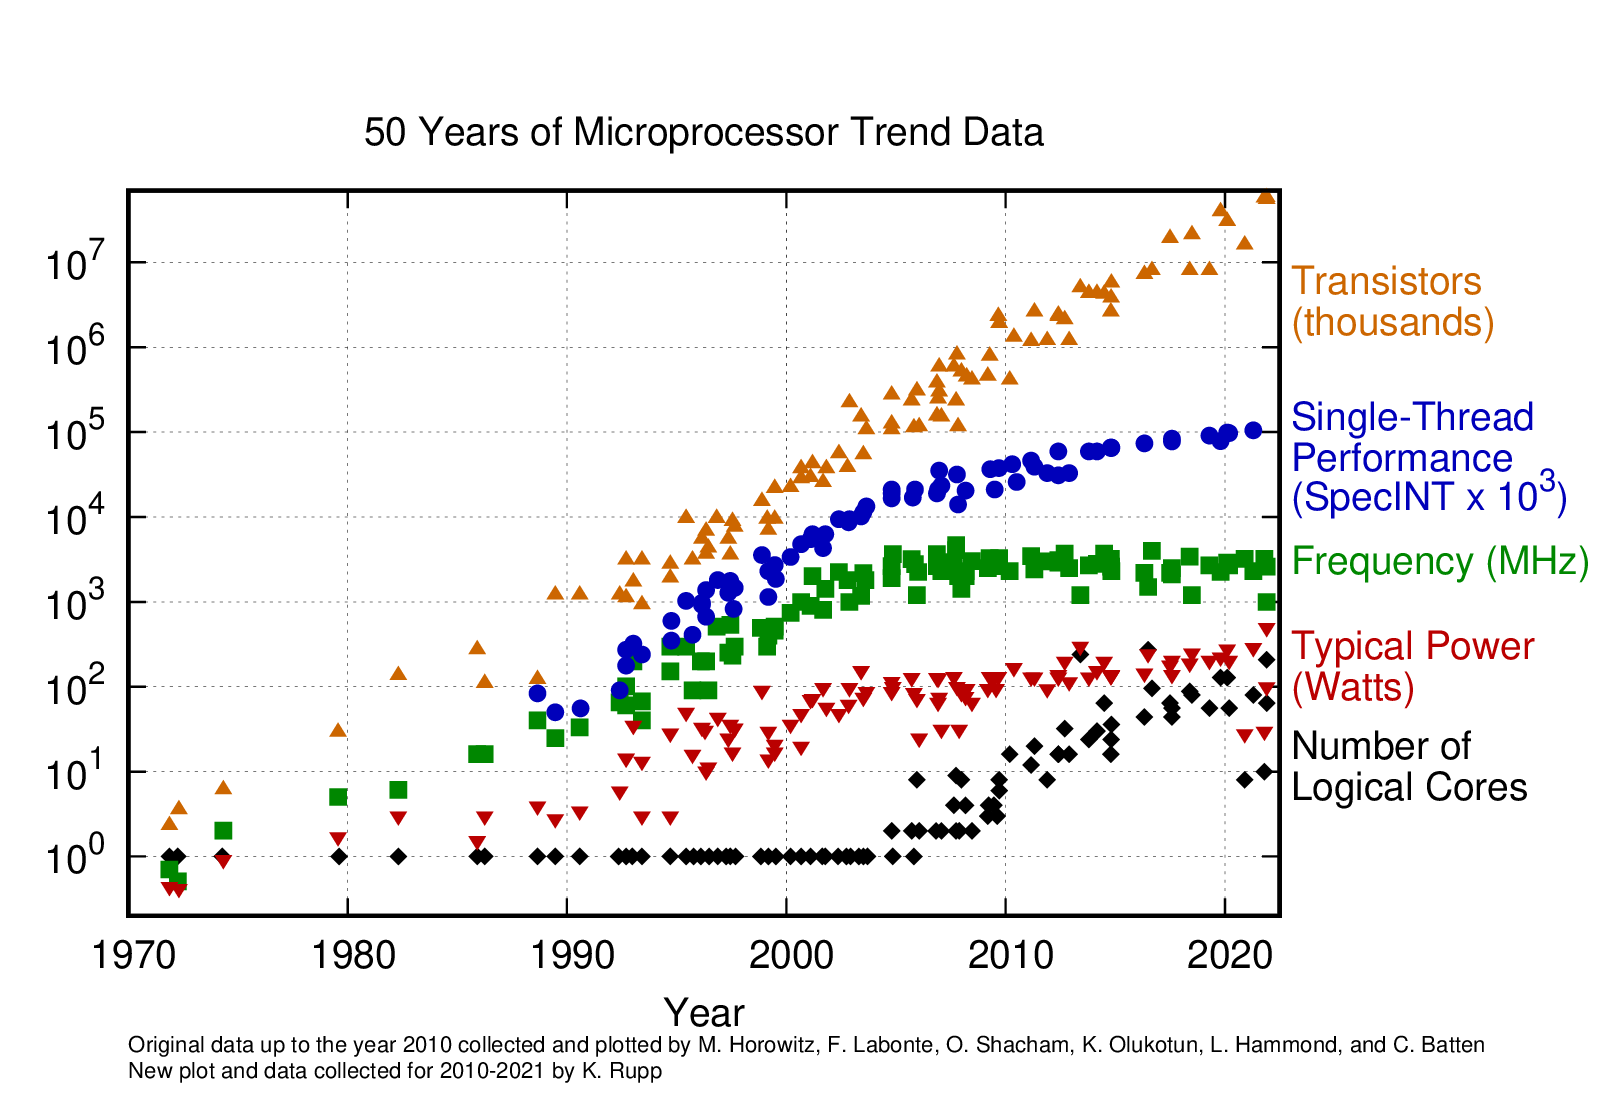
\includegraphics[width=\linewidth]{images/50-years-processor-trend.png}
	\caption{Trends of microprocessors.}
	\label{fig:processor-trend}
\end{figure}

This particular moment (around 2006) is known as ``Hit the \textit{Power Wall}'' \cite{Bose:2011:Power}.
At that time, the performance improvements of uniprocessors had come to an end due to power constraints.
This was a clear indicator that other factors have to be modified in order to gain an increase in performance. The next step is to invest on parallel architectures.

On the other hand, in the scientific and technological field, HPC is a great tool that helps researchers.
It allows the simulation of complex environments and systems (useful in physics, biology, chemistry, etc.) and the performance of intensive calculations of long duration in conventional computers, among other applications.
Due to its great time efficiency and the variety of areas of knowledge in which HPC can be used, the potential for the study of parallel computing and its application in high performance computing is clear.

There has been interest in parallel computation for a long time.
In fact, parallel computers existed before 1980 (more in-depth on page 14 of \textit{"Parallel Computing Works!"} \cite{Fox:2014:Parallel}), but greater achievements on the field were accomplished later on. Nowadays, there is a wide variety of devices for different kinds of computation objectives (CPU, FPGA, GPU, ASIC, etc.).
It has become an heterogeneous world full of distinct architectures. As a matter of fact, it has been claimed that we are currently in \textit{``A New Golden Age for Computer Architecture''} \cite{Hennessy:2019:New}.

The reasons behind the different specializations is to optimize for a particular kind of task.
This entails a more effective use of memory bandwidth and increased performance from the deliberate elimination of unnecessary accuracy, among other advantages.

With the vast amount of available devices comes the also varied collection of APIs and other utilities regarding the use of both hardware and software.
Some relevant abstraction mechanisms for parallel work include CUDA\footnote{\href{https://developer.nvidia.com/cuda-zone}{{CUDA Library of Resources} \url{https://developer.nvidia.com/cuda-zone}}}, OpenMP\footnote{\href{https://www.openmp.org}{{OpenMP API specification} \url{https://www.openmp.org}}}, OpenCL\footnote{\href{https://www.khronos.org/opencl/}{{OpenCL Main Page} \url{https://www.khronos.org/opencl/}}} and specially SYCL \cite{URL::SYCL}, but keep in mind that this is nowhere near the total amount of tools that provide this service.

This situation is quite problematic because this heterogeneous world requires heterogeneous solutions and tools.
This means that, in order to produce code that is targeted towards multiple back-ends or devices, there needs to be an abstraction that permits to do so, allowing multiple tools to work together.
Moreover, regarding HPC, both hardware and software abstraction utilities may allow for an easier way of expressing scalability, portability and versatility.
This begs for a tool that provides a more generalistic yet time and performance efficacious approach. In response to this situation comes SYCL.

% \section{SYCL overview}

SYCL is a single source, high-level, standard C++ programming model, that can target a range of heterogeneous platforms.
There are many back-end implementations that support SYCL (Fig. \ref{fig:sycl-implementations}).
We are going to focus on the Intel DPC++ branch\footnote{\href{https://github.com/intel/llvm}{{Intel oneAPI DPC++ compiler} \url{https://github.com/intel/llvm}}}.

\begin{figure}[H]
	\centering
	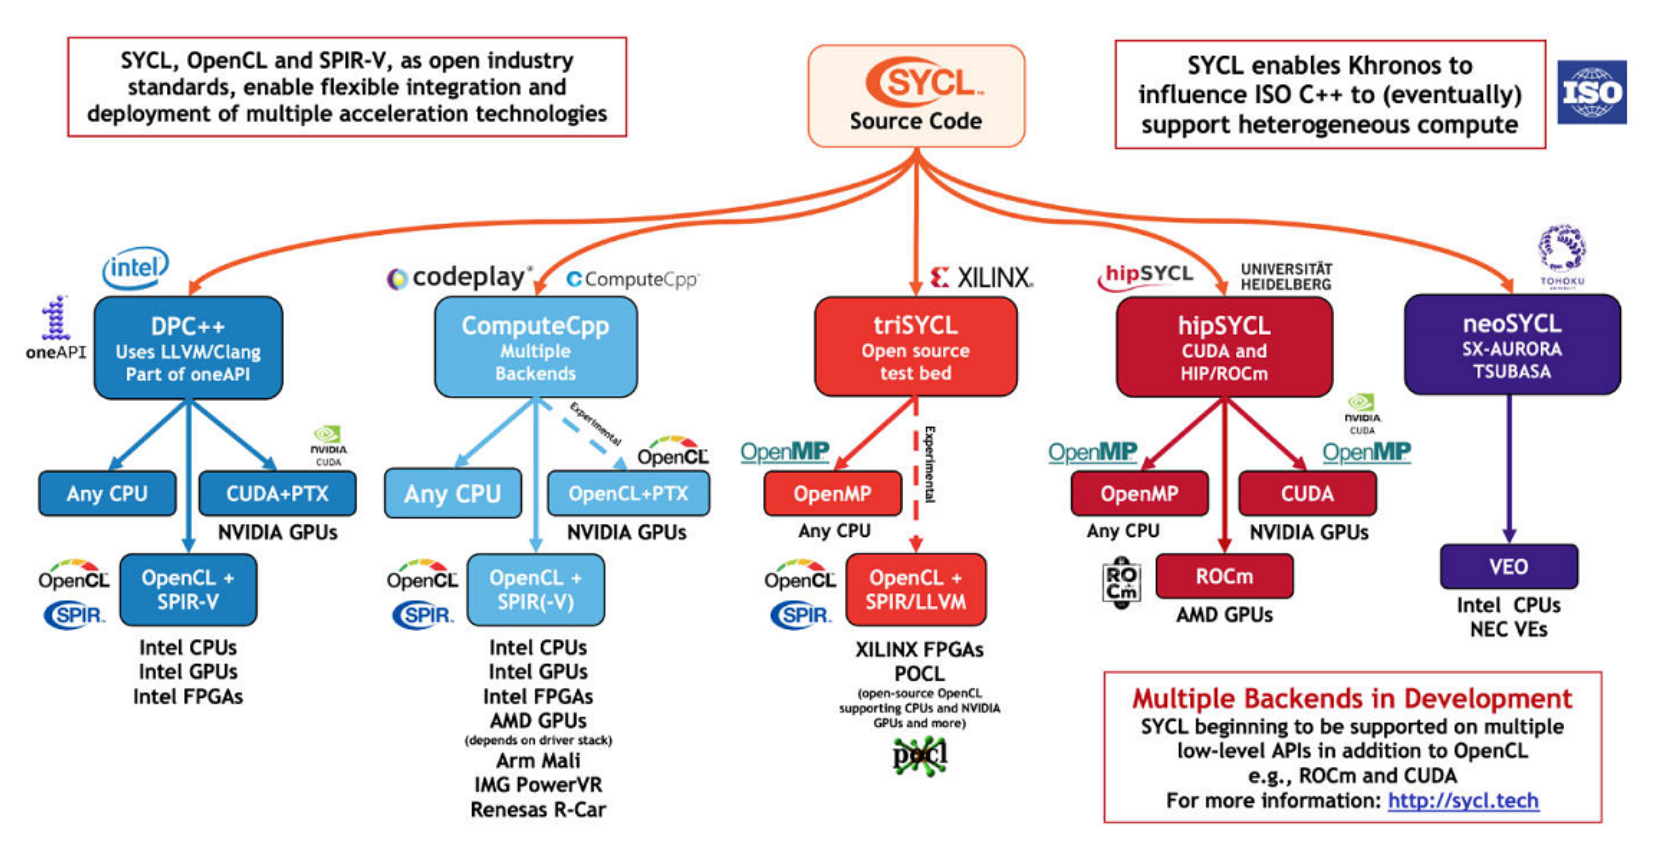
\includegraphics[width=\linewidth]{images/sycl-implementations.png}
	\caption{SYCL implementations.}
	\label{fig:sycl-implementations}
\end{figure}

This work aims to perform a deep exploration of SYCL and its capabilities, as well as producing benchmark tests with other platforms such as CUDA.
Another topic of interest is the analysis and implementation of different data management models.
As a given, this study will be covering these tasks from a HPC perspective when possible.

All the code examples written by the student for this work follow the principles of Martin's Clean Code book \cite{Martin:2009:Clean} and conform to the Google's Style Guide\footnote{\href{https://google.github.io/styleguide/}{{Google Style Guides} \url{https://google.github.io/styleguide/}}}, while code excerpts from other works will remain essentially untouched.
The reason behind the decision to write code using Google's Style is completely arbitrary, the importance of choosing a style relies on being consistent with its use: \textit{``The last thing we want to do is add more complexity to the source code by writing it in a jumble of different individual styles.'' - Robert C. Martin}.

Every piece of code written by the student for this project is publicly available on the GitHub repository dedicated to this work \cite{URL::TFG}.
Also note that every listing has a link to its original source and in the case of the student's code, there will be a direct link to the corresponding file in the work's repository, labeled as \textit{``See on GitHub''}.

%
% ---------------------------------------------------
%
% Proyecto de Final de Carrera:
% Author: Álvaro Fontenla aluXXX@ull.edu.es
% Chapter: Goals 
% File: Cap1_Goals.tex
%
% ----------------------------------------------------
%


\chapter{Goals} \label{chap:Goals}  
This document summarizes the research and development work carried out by the student in the achievement of his Final Degree Project (\textit{Trabajo de Fin de Grado}, TFG), which will conclude his studies for the degree \textit{Grado en Ingeniería Informática} at the \textit{Escuela Superior de Ingeniería y Tecnología} at the Universidad of La Laguna (ULL).

This project has the following main goals:

\begin{enumerate}
\item A first objective has been 

\item Finally, after the corresponding research and information gathering, the student is expected to apply the acquired knowledge to develop some functional implementation that meets the proposed needs.
\end{enumerate}

% ---------------------------------------------------
%
% Trabajo de Fin de Grado. 
% Author: Adriano dos Santos Moreira <alu0101436784@ull.edu.es>
% Chapter: Related Technologies
% File: Cap2_Related_Technologies.tex
%
% ----------------------------------------------------
%

\cleardoublepage
\chapter{Related Work} \label{chap:Related_Technologies}

Given the growing relevance of heterogeneous distributed memory systems and the large
development effort they pose nowadays, the research community has come up with a number of
interesting proposals to facilitate their usage \cite{Agullo:2017:Achieving, Sainz:2014:Leveraging,Lawlor:2009:Message,Stone:2010:OpenCL,Kim:2012:SnuCL}.
Although this work mainly covers the SYCL platform applied to HPC, it is also important to have an overview of the various approaches for parallel computing and related technologies.
There has been several developments in this field such as the ones cited above, although we are not going to discuss all of them.

This chapter is intended to make us aware of the general sense regarding the basic logic behind parallel oriented APIs and tools.
Inherently from one abstraction to another, we will see similarities within their core, revealing crucial mechanisms of parallel reasoning as well as establishing a connection between abstract procedures and physical parallel-oriented devices.

\section{OpenMP}
OpenMP\footnote{\href{https://www.openmp.org}{{The OpenMP API specification for parallel programming} \url{https://www.openmp.org}}} is the predominant API used to manage shared-memory parallelism used in scientific applications \cite{Luecke:2015:Fast}.
It allows for more efficient load balancing for multithreaded tasks.
This abstraction is also designed to be a flexible standard, so it becomes easy to implement on different platforms.
In essence, OpenMP extends C/C++ and Fortran with compiler directives and runtime functions that allow for a high level of parallelism expressiveness \cite{Dagum:1998:OpenMP}.
It is composed of the following basic ideas:
\begin{itemize}
    \item Control structure: Reduced amount of control structures, enough for most parallel applications.
    \item The data environment: Environment context for each process.
    \item Synchronization:
    \begin{itemize}
        \item \textbf{Explicit} synchronization using interprocess communication, which is slow.
        \item \textbf{Implicit} synchronization present when starting and finishing parallel and control constructs.
        \item OpenMP also offers different \textbf{tools for synchronization}, depending on the specific action and/or conditions, which are usually more time efficient than explicit synchronizations.
    \end{itemize}
    \item The runtime library: A miscellaneous set of mechanisms to tune an application, such as dynamically changing the number of processes used to execute parallel regions.
\end{itemize}

Listing \ref{listing:openmp-simple} presents a simple OpenMP application which runs a parallel for loop written in C++.

\lstinputlisting[language=C++,style=cppstyle,caption={Consecutive pairs average on OpenMP. \href{{https://www.openmp.org/wp-content/uploads/OpenMP3.1-CCard.pdf}}{\textit{Original source}}.},label={listing:openmp-simple}]{listings/openmp_simple.cc}

The purpose of the function is to calculate the average of each pair of consecutive elements in the \textit{a} array and store the result in the corresponding position of the \textit{b} array.
The OpenMP directive \texttt{\#pragma omp parallel for} is used to parallelize the loop.
As noted in the example code, the loop counter \textit{i} is implicitly private in OpenMP, meaning that each thread gets its own private copy of \textit{i}.

\section{HPL}

The HPL (Heterogeneous Programming Library) \cite{Viñas:2018:Heterogeneous} is a framework built on top of OpenCL that enables the exploitation of heterogeneous computing in C++.
Within HPL, the primary application operates on the host, and the code segments executed in OpenCL consist of kernel functions.
These functions can be written either directly in C++ using the HPL embedded language or in native OpenCL C.

The main functionality of this library comes with its \texttt{Array} class, which encapsulates the data to be manipulated inside of the kernels, indicating both the data type and the number of dimensions of the array.
On the other hand, scalar types should also be encapsulated within their HPL equivalent (\texttt{Float}, \texttt{Int}, etc.).
Listings from this section illustrate these ideas.

\lstinputlisting[language=C++,style=cppstyle,caption={SAXPY on HPL (HPL embedded language). \href{{https://github.com/fraguela/hpl?tab=readme-ov-file}}{\textit{Original source}}.},label={listing:hpl-saxpy-embedded}]{listings/hpl_saxpy_embedded.cc}

Listing \ref{listing:hpl-saxpy-embedded} displays how to perform a SAXPY (single precision A X plus Y) operation using the HPL embedded language.
To create a kernel we simply write a regular C++ function and use the data types provided by the library as the argument types.
To invoke the kernel, we call the \texttt{eval()} function with the kernel name as the argument followed by another call with the arguments for the execution of the kernel, as shown in Listing \ref{listing:hpl-saxpy-embedded}

Since this platform is based on OpenCL, there is a method to execute already coded OpenCL kernels.
Listing \ref{listing:hpl-saxpy-opencl} exemplifies this case.
The key difference from the former example remains on the procedure for the kernel call.
Just before the \texttt{eval()} call, we associate the OpenCL version of the kernel (specified in the \texttt{saxpy\_kernel} string) with the HPL function handle via the \texttt{nativeHandle()} function, which arguments are a function whose arguments define an equivalent version of the kernel written as specified for the HPL framework (additional details regarding the kernel behaviour can be specified), the name of the kernel function within the code and the actual OpenCL code.
\pagebreak

\lstinputlisting[language=C++,style=cppstyle,caption={SAXPY on HPL (OpenCL kernel). \href{{https://github.com/fraguela/hpl?tab=readme-ov-file}}{\textit{Original source}}.},label={listing:hpl-saxpy-opencl}]{listings/hpl_saxpy_opencl.cc}

\section{CUDA}

As presented in \cite{Liang:2011:GridCuda}, CUDA\footnote{\href{https://docs.nvidia.com/cuda}{{CUDA C++ documentation} \url{https://docs.nvidia.com/cuda}}} is a programming model and a parallel computing platform developed by NVIDIA, aimed to be used in general purpose GPUs for their CUDA-enabled GPU devices.
It was originally launched in 2007 and one of its main goals is to allow for the creation of scalable programs within the parallel computing paradigm.
To accomplish this, CUDA offers a simple yet powerful abstraction based on three key points: a hierarchy of thread groups, shared memories and barrier synchronization.

\begin{figure}[H]
	\centering
	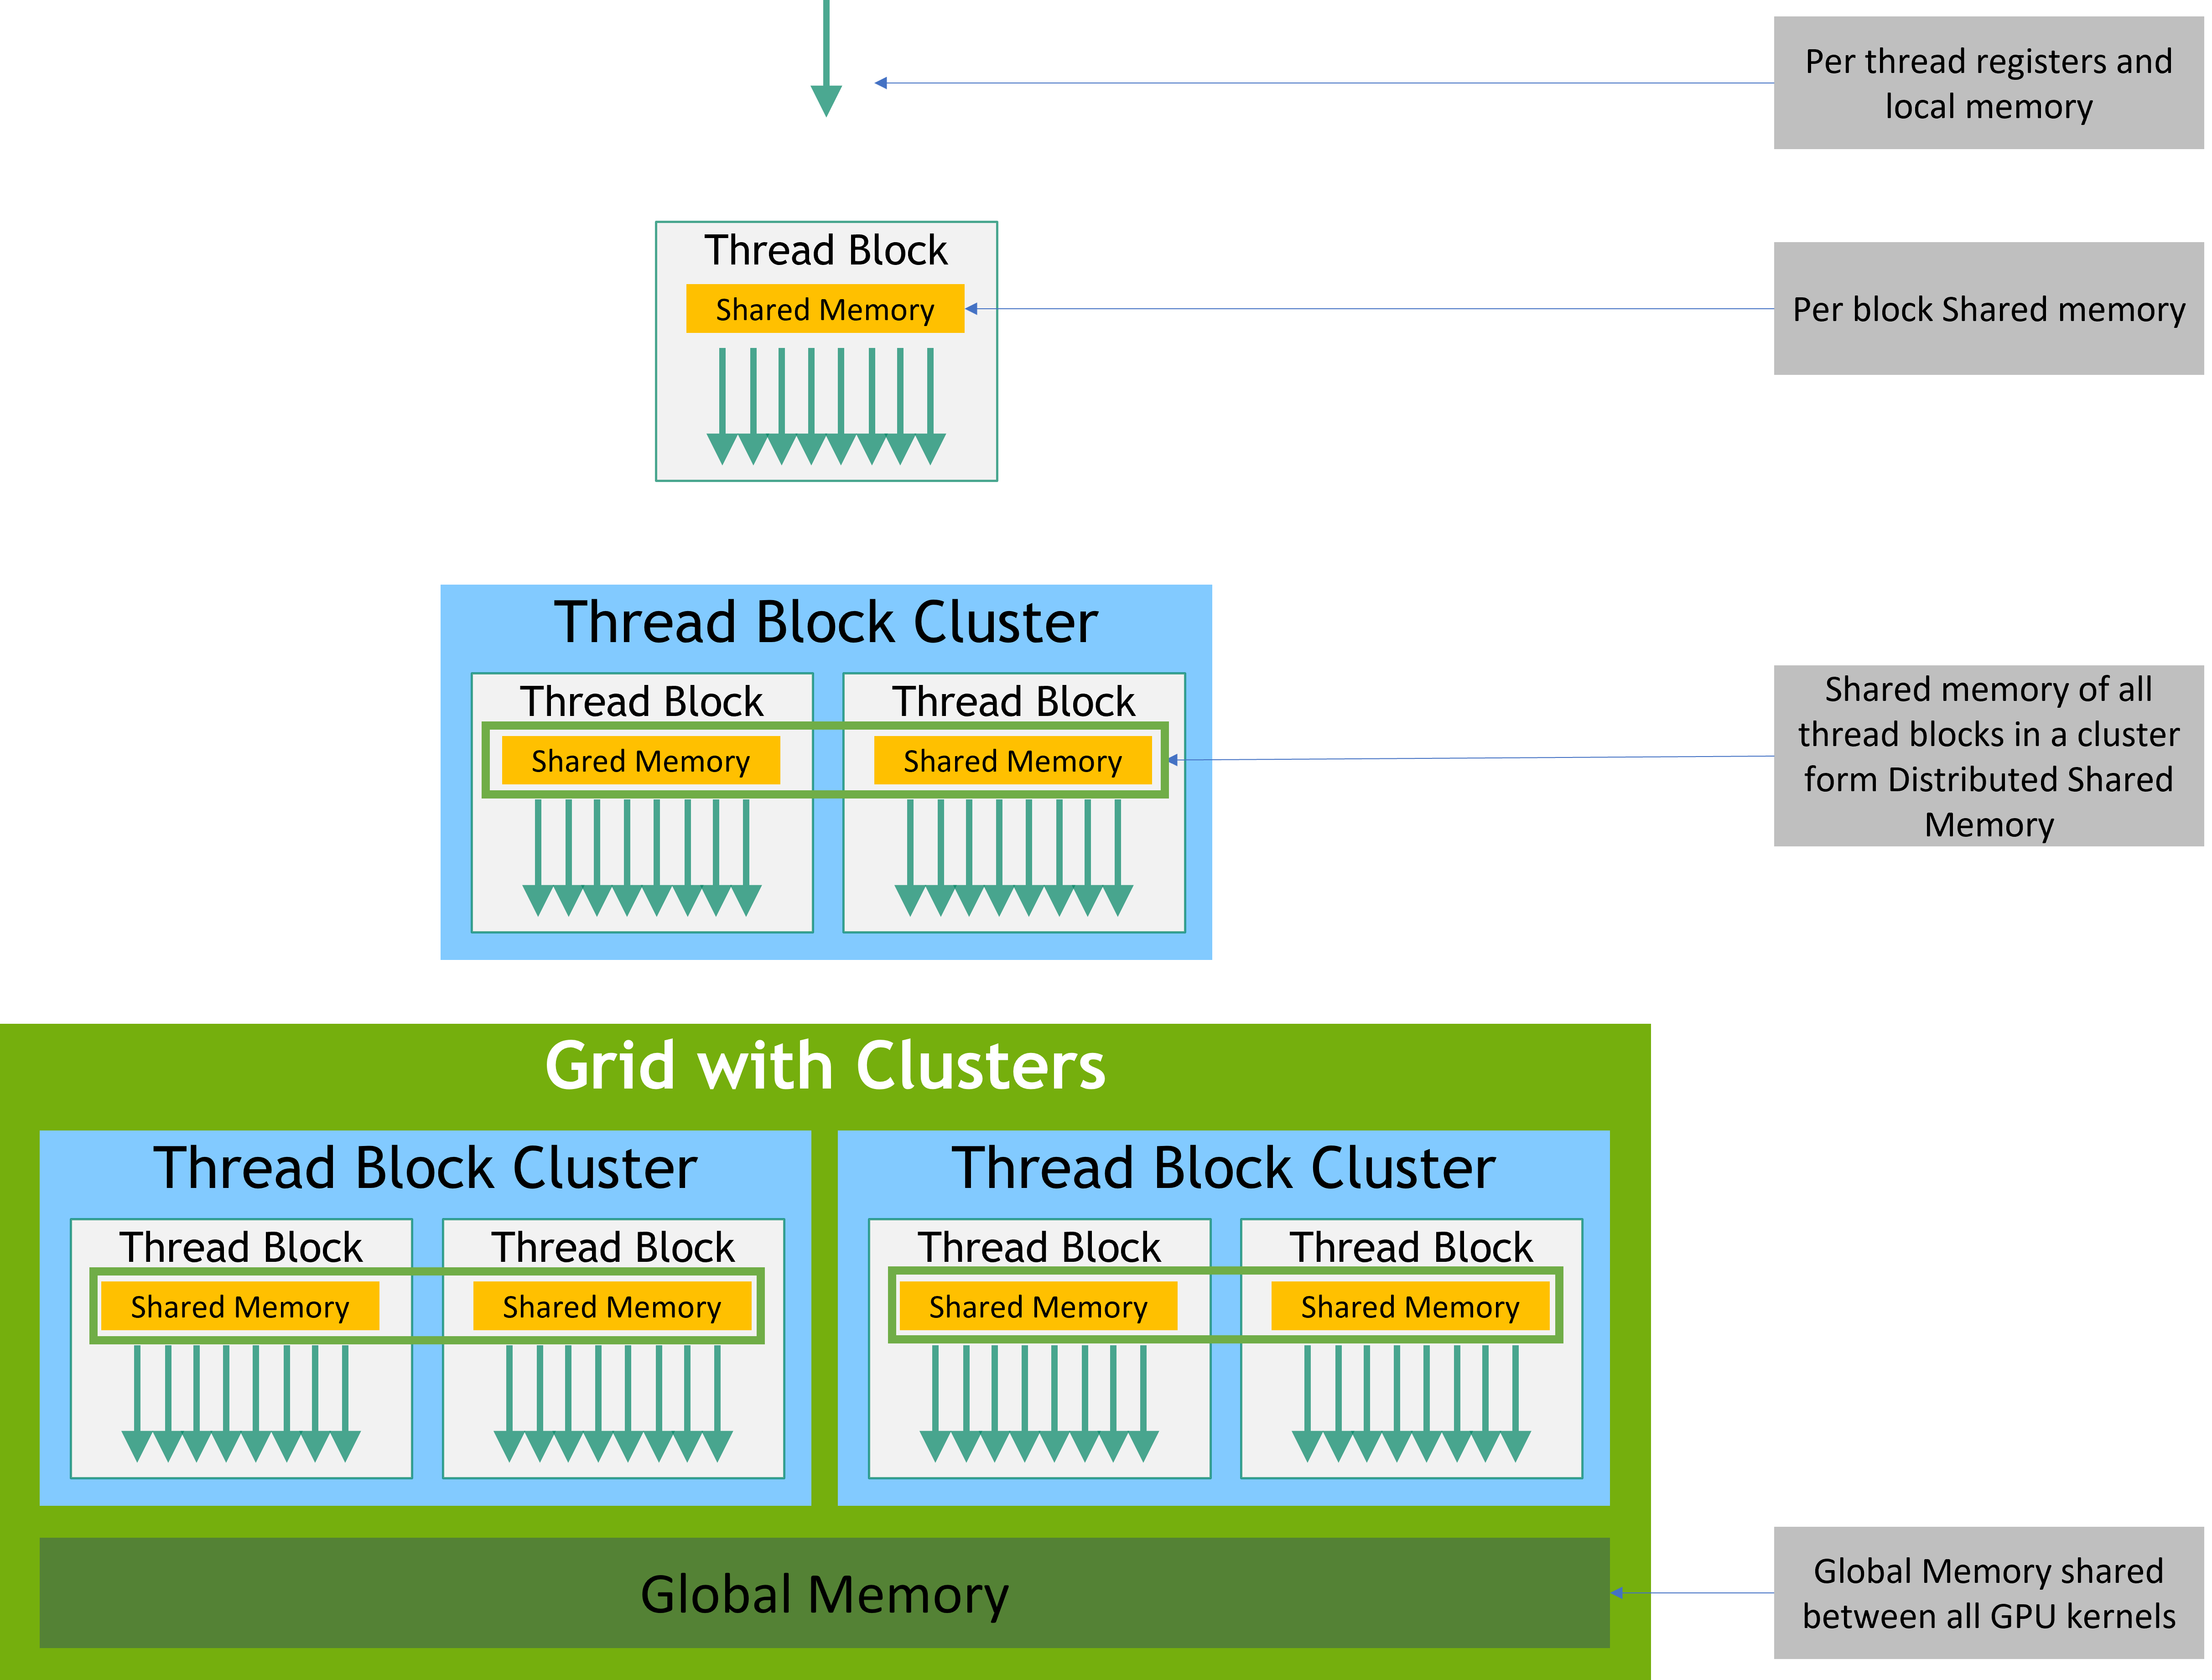
\includegraphics[width=\linewidth]{images/cuda-memory-hierarchy.png}
	\caption{CUDA memory hierarchy.}
	\label{fig:cuda-memory-hierarchy}
\end{figure}

With the CUDA platform, problems can be subdivided in blocks of threads within a grid and subproblems can be solved in parallel cooperation within a block.
The memory system in place for all of these pieces works as shown in Figure \ref{fig:cuda-memory-hierarchy}
The division in multiple independent pieces allows for scheduling on an undetermined number of GPU processors, thus enabling hardware scalability.
This platform is used broadly to solve real world problems regarding physics, biology and data mining, among others.

The CUDA platform is available on a wide variety of languages, primarily focusing on C/C++ and Fortran.
To display the basic usage and expressions for CUDA, we present in Listing \ref{listing:cuda-vector-add} an example program written in C++.
\pagebreak

\lstinputlisting[language=C++,style=cppstyle,caption={Vector add on CUDA. \href{{https://docs.nvidia.com/cuda/cuda-c-programming-guide/index.html\#kernels}}{\textit{Original source}}.},label={listing:cuda-vector-add}]{listings/cuda_vector_add.cc}

First of all, we have a declaration of a function starting with the \texttt{\_\_global\_\_} keyword, which specifies the following function as a kernel, which can only be executed on the device.
Inside of it there is the actual kernel code, in which we can highlight the use of \texttt{threadIdx}, a 3-dimensional vector which identifies the working thread.

Similarly, we have \texttt{blockIdx} that provides a unique identification for thread blocks.
On the other hand, inside of the main function there is a kernel invocation.
This asynchronous call comes with execution configuration denoted by \texttt{<}\texttt{<}\texttt{<1, N>}\texttt{>}\texttt{>}, in which the first parameter specifies the number of blocks and the second specifies the number of threads per block.
Both of which can be simple integers or \texttt{dim3} values to indicate these are multidimensional entities.

\section{OpenCL}

OpenCL is an open standard designed for general-purpose parallel programming on multi-core architectures \cite{Viñas:2018:Heterogeneous, Reyes:2012:Directive}.

It addresses a wide range of applications and acts as an efficient, low-level programming interface. The goal of OpenCL is to establish itself as the foundation platform for a parallel computing ecosystem.
OpenCL aims to be a tool to produce portable yet efficient code.
There is a clear division of ideas that comprehend the standard, which is composed of the models: Platform, Memory, Execution and Programming.
These are explained in further detail in the reference above.
Following, we have an overview of the OpenCL functionality.

\begin{figure}[H]
	\centering
	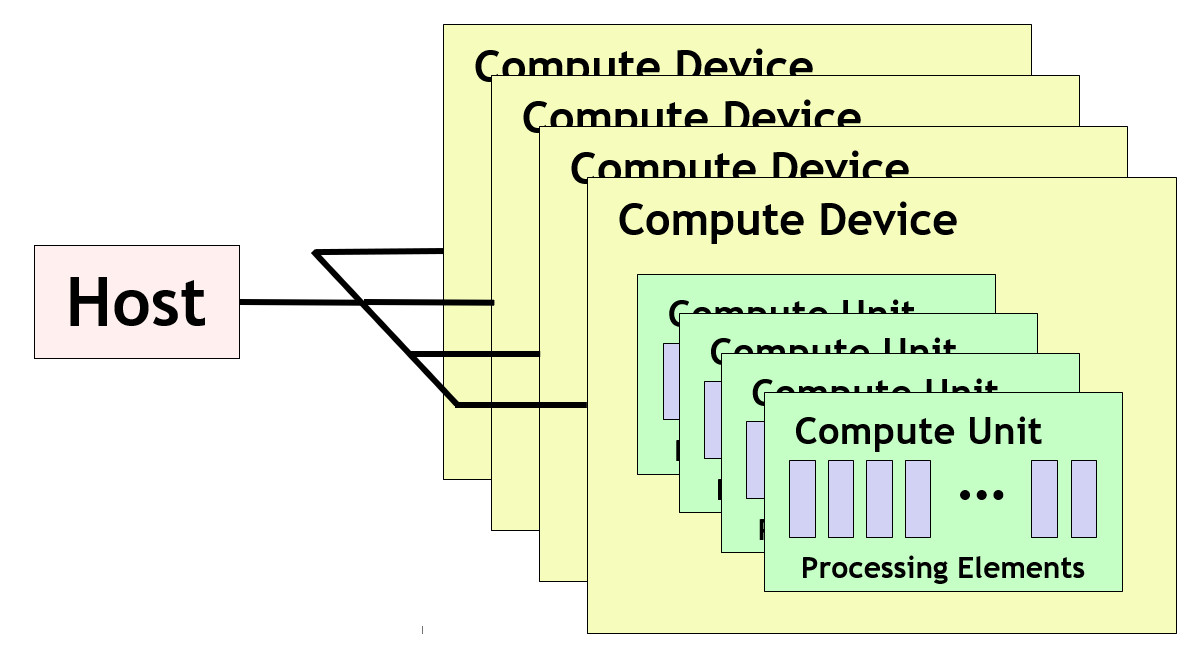
\includegraphics[width=0.7\linewidth]{images/opencl_platform_model.jpg}
	\caption{OpenCL platform model.}
	\label{fig:opencl-platform-model}
\end{figure}

As we can see in Figure \ref{fig:opencl-platform-model}, an OpenCL host is connected to one or more OpenCL devices, which in turn are composed of one or more compute units (CU).
Such units are subdivided in one or more processing elements (PEs).
The PEs are the ones in charge of executing actual code.

The way an OpenCL application operates is by running the host program on the host platform, which is in charge of defining the kernel contexts and managing kernel executions, whilst submitting commands from it to execute kernels on the devices.

Similarly to CUDA, kernels are scheduled to run under a defined index space, meaning that each kernel instance has a specific identification, which determines how the kernel will execute.

\begin{figure}[H]
	\centering
	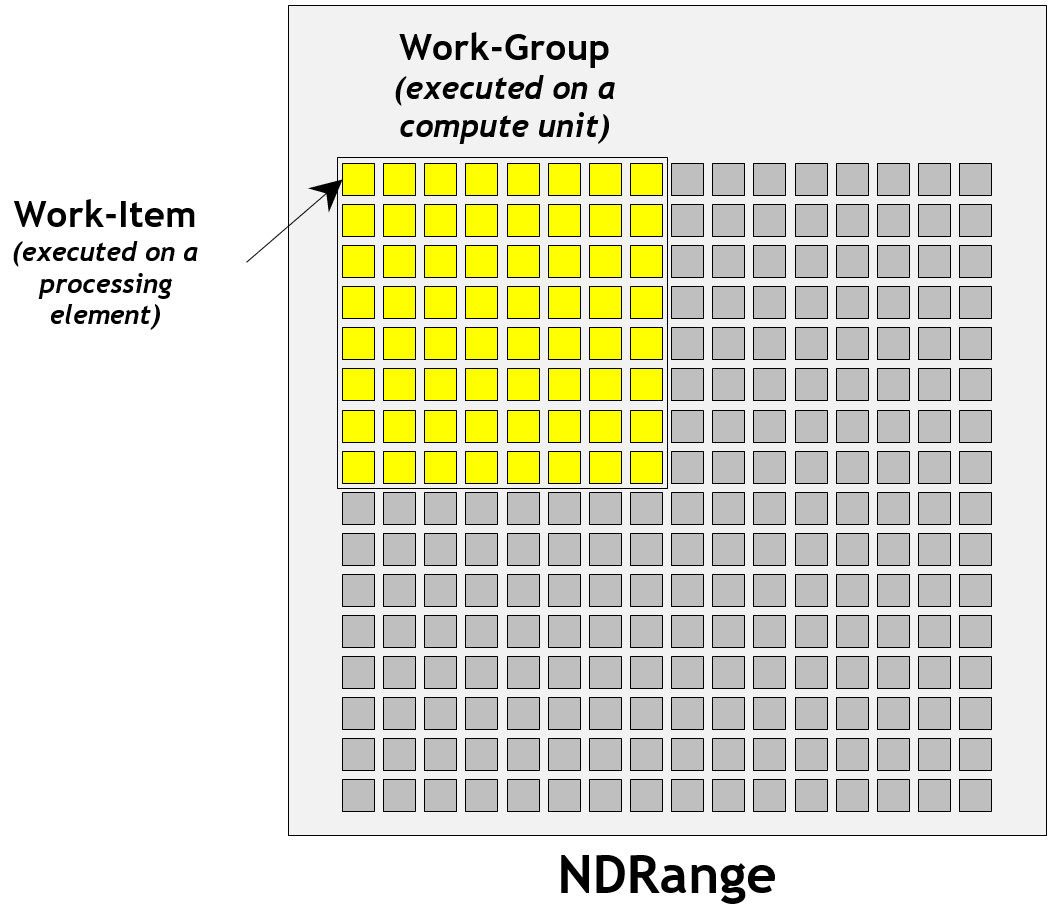
\includegraphics[width=0.75\linewidth]{images/opencl-ndrange.jpg}
	\caption{OpenCL NDRange.}
	\label{fig:opencl-ndrange}
\end{figure}

A PE is responsible for the execution of a work-item, which is encompassed within a work-group, as we can see in Figure \ref{fig:opencl-ndrange}.
This coarse-grained composition allows for the execution of different strategies when using the index space.
Furthermore, the idea of a N-dimensional index space (NDRange), where N is one, two or three, gives users high flexibility to refine their works.
This abstraction shapes the indexes used in the work-items, affected by the dimensionality and work group divisions as well.

\section{Directive-based Languages for Accelerators}

In \cite{Grillo:2013:PGD}, the authors present the most relevant approaches that have been used to leverage heterogeneous architectures using languages enhanced with the use of specific directives.

We will now review the most significant of these approaches.

\subsection{OpenMPC - OpenMP Extended for CUDA}

OpenMPC \cite{Lee:2010:OpenMPC} is an abstraction of the CUDA programming model built on OpenMP.
OpenMPC performs a translation from OpenMP to CUDA with the addition of special directives and variables, which are used to make CUDA-specific optimizations.
There is an extensive set of clauses and environment variables.
Examples of some of these clauses are:
\begin{itemize}
    \item \texttt{maxnumofblocks(N)}: Specifies the maximum number of thread blocks for a kernel.
    \item \texttt{threadblocksize(N)}: Specifies the thread block size for a kernel.
\end{itemize}
The translation from OpenMPC to CUDA starts by analyzing the code and passing the result to the OpenMP to CUDA translator, which performs the actual translation aided by the optimization information obtained from the previous step.

\subsection{hiCUDA}

hiCUDA \cite{Han:2011:hiCUDA} is a high-level abstraction layer built on top of CUDA.
It provides an easy to use interface that solves mechanical tasks for the development of CUDA programs.
An important highlight that motivates the use of hiCUDA is the fact that the process of migration from existing code to CUDA may be challenging, as evidenced by the need for programmers to manually handle intricate tasks such as managing data transfers between host and GPU memories, and optimizing GPU memory utilization.
These tedious tasks are alleviated by the automated work that hiCUDA can offer.

This tool can extract kernels from their original source and decide how to allocate the work threads and blocks according to user defined configuration clauses.
This is accomplished using special hiCUDA directives, which would then be translated to actual CUDA code.
The authors have developed a prototype of this idea which does exactly that.
Is also important to note that the same source files of a hiCUDA project can be used to create both sequential and GPU versions of the code.

\subsection{PGI Accelerator Model}

The PGI Accelerator Model \cite{Portland:2010:PGI} was created by The Portland Group for the Fortran and C languages.
It is essentially a set of directives designed to guide the compiler in creating kernels and regions of code that can be offloaded to an accelerator device.
This model allows for portability across multiple operating systems, various accelerators and types of host CPUs.

The main functionality is provided by the \texttt{acc region} directive, which specifies a region within the code that contains a parallel loop kernel.
Most of the directives provided by this model are optional, and are mostly used to improve performance based on compilation hints.
On the other hand, this abstraction offers implicit mechanisms such as data flow and array region analysis to determine when data transfers between host and device should occur, as well as accelerator startup and shutdown, among other uses.

\subsection{OpenACC}

Considering the OpenACC standard, the ULL GCAP\footnote{\href{https://portalciencia.ull.es/grupos/6369/detalle}{{ULL GCAP} \url{https://portalciencia.ull.es/grupos/6369/detalle}}} research group (\textit{High Performance Computing Group}) developed their own version of the compiler, called \texttt{accULL} \cite{Reyes:2012:Directive}, standing as one of the few available implementations of the OpenACC standard.
OpenACC shares an important piece of the high-level features present in the PGI Accelerator Model, it is based on directives that indicate regions of code that could be run on an accelerator device.
This abstraction frees the developer from writing device specific code details, allowing them to focus on other tasks.
The main \textit{pragma} regions supported by OpenACC are the following:
\begin{itemize}
    \item \texttt{data}: Specifies data regions.
    \item \texttt{kernels}: Groups of loop nests that can be executed on the devices.
    \item \texttt{parallel}: Similar to \texttt{kernels} but allows for better control over the code.
\end{itemize}

There are other annotation mechanisms to further tailor the execution and behaviour of OpenACC such as clauses that can reduce memory transfers like \texttt{copy\_in} or \texttt{copy\_out}.

%
% ---------------------------------------------------
%
% Proyecto de Final de Carrera:
% Author: Adriano dos Santos Moreira <alu0101436784@ull.edu.es>
% Chapter: SYCL
% File: Cap3_SYCL.tex
%
% ----------------------------------------------------
%


\chapter{SYCL} \label{chap:SYCL}

In this chapter we will take a deep dive into the mechanisms and abstractions that the SYCL platform offers.

We chose \textit{Data Parallel C++} \cite{Reinders:2023:Data} as the baseline book to learn about SYCL.
It is a very recently published reference for this platform (first edition published in November 2020, second in October 2023) that also serves as an introduction to parallel programming, as it introduces the very basic concepts and builds on them in a beginner friendly manner.
On the other hand, SYCL Academy\footnote{\href{https://github.com/codeplaysoftware/syclacademy}{{SYCL Academy} \url{https://github.com/codeplaysoftware/syclacademy}}} fills the need for a more practical approach for an introduction to SYCL, offering a 20 lectures long tutorial, containing both lessons and exercises.

Based on the study of the mentioned sources, in the following sections we will cover the foundational ideas and procedures contained in the SYCL platform.

Nevertheless, this chapter does not aim to provide an exhaustive explanation of SYCL and its programming API.
For a deeper understanding, the interested reader is referred to the above references, also including the SYCL technical specification \cite{URL::SYCL-Specification}.

\section{What is SYCL?}

SYCL is a parallel focused abstraction layer created for C++. Although the idea of a mechanism that provides tools for parallelism existed for a long time, the unique trait of SYCL is that it attempts to define a uniform protocol for parallel execution.
In such a way, it allows for portable programmability across multiple vendors and platforms. Thus, bringing to existence a powerful tool which fulfils the following statement from \textit{Parallelizing the Standard Algorithms Library} \cite{Hoberock:2012:Parallelizing}:

\vspace{3mm}
\textit{``...standard and broadly-accessible functionality should be constructed to bridge the gap between the abundant parallelism implicit in many applications and the concurrent resources of the target architecture...''} 
\vspace{3mm}

This is a notable effort since these features were desired for almost a decade by the time SYCL 2020 was launched.

It is worth mentioning that SYCL has some similarities to OpenCL, sharing concepts and terminology like NDRanges and command queues (called just queues in SYCL).
In fact, when SYCL was created it was an abstraction layer only for OpenCL, and later it was expanded to support multiple back-ends in SYCL 2020.

Having stated what SYCL is, we will review a simple SYCL program that performs a scalar addition so we can grasp how a minimal SYCL operates.
In the first line of Listing \ref{listing:scalar-add} we have the inclusion of the SYCL header file.

\lstinputlisting[language=C++,style=cppstyle,caption={Scalar add example using the buffer/accessor model. \href{{https://github.com/AdrianoMoreira08/TFG-SYCL/blob/main/sycl-examples/scalar_add.cc}}{\textit{See on Github}}.},label={listing:scalar-add}]{listings/scalar_add.cc}

This code performs the sum of \texttt{summand\_a} and \texttt{summand\_b}, writing the result in the \texttt{result} variable.
On line 6 we have the key object of any SYCL program, the queue.
It allows for communication between host and device and execute various operations.
Lines 8-10 define buffers to manage the previously stated data.

Then we have a call to \texttt{submit} in line 12, which schedules a \textit{command group} to be executed.
Which is, to simplify, a set of arbitrary code and a kernel execution call.
This is the first step to get actual kernel code executing on a device.

Inside this command group there are three \textit{accessors}, which grant access to the buffers within the kernel.
On lines 17-19 there is the kernel definition and invocation.

In the next sections of this chapter we will cover the details and unexplained elements of this example.

\section{The Queue}

Queues\footnote{\url{https://registry.khronos.org/SYCL/specs/sycl-2020/html/sycl-2020.html\#sec:interface.queue.class}} are the main piece of action in SYCL.
They allow the host program to communicate with an underlying device or devices.
An instance of a queue is connected to one device and can execute different operations concerning the device itself and between host and device.
Note that multiple queues can be bound to the same device but one queue is only bound to a single device.
Another point to mention is that the SYCL host program can be executed on any type of physical device as long as it supports C++17, although is often going to be executed on a CPU.

\subsection{Task Graph}

SYCL organizes the work to be performed using a dependency graph.\footnote{\url{https://registry.khronos.org/SYCL/specs/sycl-2020/html/sycl-2020.html\#sec:command-groups-exec-order}}
Each node of the graph represents a unit of work, and the edges between them symbolize either custom or automatically set dependencies, as the example shown in Figure \ref{fig:dependency-graph}.

\begin{figure}[H]
    \centering
    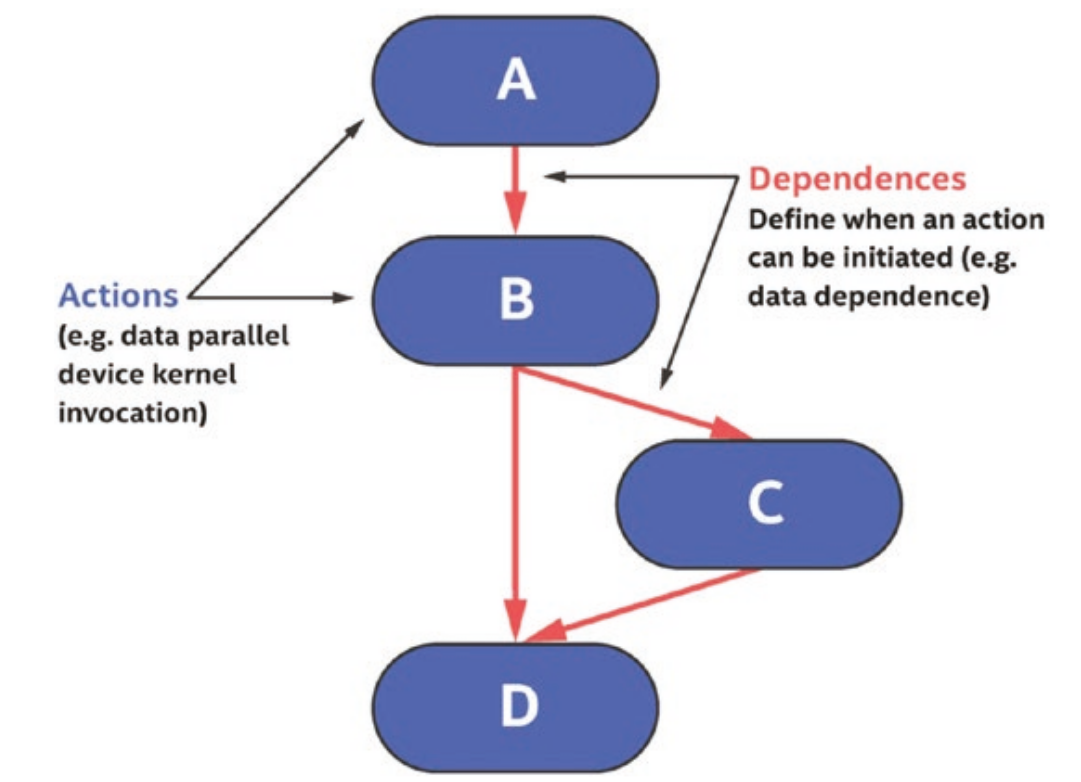
\includegraphics[width=0.7\linewidth]{images/dependency-graph.png}
    \caption{Dependency graph example. \textit{Image From Data Parallel C++} \cite{Reinders:2023:Data}}
    \label{fig:dependency-graph}
\end{figure}

With this structure, it is easy to determine which actions come next, as well as ensuring that the work is safe to execute.
SYCL automatically sets dependencies when working with the buffer/accessor model, as it provides the runtime with information regarding the use of the data present in the buffers.
On the other hand, in the Unified Shared Memory (USM) model, which is based on memory pointers, there is automatic data dependency management only when using certain types of pointers.
It is also possible to create dependencies manually.

\subsection{Device Selection}

When creating a queue, a device is assigned to it.
If nothing is specified, the runtime will select a device without taking into consideration the program needs, which can result in a device selection lacking the features the code requires.
SYCL will always guarantee that at least one device is available.

There are methods\footnote{\url{https://registry.khronos.org/SYCL/specs/sycl-2020/html/sycl-2020.html\#sec:device-selector}} to choose a specific device or with specific characteristics.
The functions \texttt{cpu\_selector\_v} (as seen on Listing \ref{listing:cpu-selector}) and \texttt{gpu\_selector\_v}, among others, are built-in selectors that can be passed as a parameter to the queue constructor to request for a certain type of device.
If device selection fails, the selector throws a \texttt{runtime\_error} exception.
\pagebreak

\lstinputlisting[language=C++,style=cppstyle,caption={Using a CPU selector. \href{{https://github.com/AdrianoMoreira08/TFG-SYCL/blob/main/sycl-examples/cpu_selector.cc}}{\textit{See on Github}}.},label={listing:cpu-selector}]{listings/cpu_selector.cc}

A more specific approach to device selection can be done by stating \textit{device aspects} using the \texttt{aspect\_selector} function, which tries to find a device that meets the declared aspects.

There is a list of standard aspects that can be requested, some of them include: \texttt{gpu}, \texttt{host\_debuggable} and \texttt{usm\_device\_allocations}.

There is an even more precise method to select a device.
Similarly to the built-in selectors, we can create a custom callable object or function that gives a score to each device.
It is an arbitrary procedure, so any technique can be used to calculate the score.
A good approach may be to use the \texttt{get\_info()} function template to retrieve data related to the device and calculate a score based on it.

\subsection{Errors and Exceptions}

When an error occurs in SYCL, it is handled through an exception.\footnote{\url{https://registry.khronos.org/SYCL/specs/sycl-2020/html/sycl-2020.html\#sec:interface.queue.errors}}
There are two types of errors:
\begin{itemize}
    \item \textbf{Asynchronous}, which result in exceptions thrown by the SYCL scheduler and may happen on a device or when trying to launch work on a device.
    \item \textbf{Synchronous} that occur when an error condition can be identified when the host program executes an operation.
\end{itemize}
\pagebreak
\lstinputlisting[language=C++,style=cppstyle,caption={Synchronous and asynchronous error handling procedures. \href{{https://github.com/AdrianoMoreira08/TFG-SYCL/blob/main/sycl-examples/error_handling.cc}}{\textit{See on Github}}.},label={listing:error-handling}]{listings/error_handling.cc}

The way synchronous and asynchronous errors are handled differ.
A synchronous error can be caught within the host program in a similar way to the example of Listing \ref{listing:error-handling}, where the try-catch block handles the situation when something goes wrong.

On the other hand, asynchronous errors are passed on to an \textit{asynchronous handler}, a function that is called at specific points in the code.
This function can be created manually to customize its behaviour and we can find an example in line 6 of Listing \ref{listing:error-handling}.
It can be arbitrarily called using \texttt{queue::throw\_asynchronous()} (or other similar methods) and is automatically called when a queue or context is destroyed.

\section{Buffer/accessor Model} \label{sec:buffer-accessor}

Buffers are abstractions that represent an object or collection of objects.\footnote{\url{https://registry.khronos.org/SYCL/specs/sycl-2020/html/sycl-2020.html\#subsec:buffers}}
The type of the objects they manage can vary from C++ scalar types, SYCL vectors, structures and user-defined types that comply with the notion of being \textit{device copyable}, which we will not go into in detail here.

By themselves, buffers do not hold the data, they simply represent it.
This model is based on the interaction with the buffers and stating the actions to be performed on them.\footnote{\url{https://registry.khronos.org/SYCL/specs/sycl-2020/html/sycl-2020.html\#subsec:accessors}}
With this information, the runtime schedules all the necessary data transactions to perform the task.

\lstinputlisting[language=C++,style=cppstyle,caption={Scalar add example using the buffer/accessor model. \href{{https://github.com/AdrianoMoreira08/TFG-SYCL/blob/main/sycl-examples/scalar_add.cc}}{\textit{See on Github}}.},label={listing:scalar-add-2}]{listings/scalar_add.cc}

We will take the first SYCL program presented at the beginning of the chapter to explain the usage of the buffer/accessor model.
In lines 8-10 of Listing \ref{listing:scalar-add-2}, we define the buffers by passing a reference to the original variable and a \texttt{range} indicating how many items does the variable hold (if it was an array, its size would match the range).

To use the buffers we use \texttt{accessors}, located in lines 13-15.
To be created, they just need the buffer that is being accessed and the handler, as the data type of the buffers is deduced.
Then we can use the accessors as if they were the original variables.

SYCL provides data consistency and is in charge of moving the information to the places it is used when using the buffer/accessor model.
For further optimization, we can communicate to the runtime what we are planning to do with the data.
To do this, we can add a third parameter to the definition of the accessors, stating the type of operation that is going to take place, the \textit{access mode}.
In the case of the example, it would make sense to mark \texttt{in\_a} and \texttt{in\_b} as \texttt{sycl::read\_only} and the \texttt{out\_r} buffer as \texttt{sycl::write\_only}.
This example was not written in this way to prioritise readability, as this is the first contact with the model.

Finally, we need to address line 7, which references the buffer's scope.
Getting a buffer out of scope (destroying it) is one of the simplest ways of copying the data managed by the buffer back to the original variable.
After line 21, the scope of the buffers ends, resulting in a copy from wherever the most recent version of the information is to its original source.
This is one of a handful of methods that exists to retrieve information from a buffer, which include forcing an update of the original variables without destroying the buffer and using a \texttt{host\_accessor} to access the data from the host.

\section{Unified Shared Memory Model}

USM\footnote{\url{https://registry.khronos.org/SYCL/specs/sycl-2020/html/sycl-2020.html\#sec:usm}} is a pointer-based model that leverages devices that support a unified virtual address space, meaning that a host memory pointer created using USM serves as a valid pointer address in the device.
There are three types of memory allocation:
\begin{itemize}
    \item \texttt{device}: Allocation happens in device memory.
    Can be directly accessed from the device but has to be explicitly copied to the host to be accessed from there.
    \item \texttt{host}: Host allocated memory that can also be accessed from the device without an explicit copy.
    To retrieve this data from the device, it is streamed over a bus rather than copied.
    \item \texttt{shared}: Similarly to a \texttt{host} allocation, the information can be accessed from both the host and device.
    The difference is that data can migrate back and forth between host and device.
\end{itemize}
\pagebreak
\lstinputlisting[language=C++,style=cppstyle,caption={Multiple scalar additions using the USM model. \href{{https://github.com/AdrianoMoreira08/TFG-SYCL/blob/main/sycl-examples/usm_scalar_add.cc}}{\textit{See on Github}}.},label={listing:usm-scalar-add}]{listings/usm_scalar_add.cc}

The USM model offers implicit data movement using \texttt{host} or \texttt{shared} allocations, while also giving the possibility to use explicit data movement through \texttt{device} allocations.
On Listing \ref{listing:usm-scalar-add} we can see a parallel scalar addition using \texttt{shared} memory.
We observe that memory access is pretty straightforward, just as if we were using regular C++ arrays.
Although this is simple, behind the scenes there are additional schedules in place to deliver the information.
In the last lines of Listing \ref{listing:usm-scalar-add}, we free the memory using SYCL's \texttt{free} function.

\section{Work Submission}

A host program can schedule memory management tasks as well as kernel execution tasks.\footnote{\url{https://registry.khronos.org/SYCL/specs/sycl-2020/html/sycl-2020.html\#\_queue\_interface}}
These operations will always be encapsulated within a command group, which is then submitted to the queue.

The submitted work will be organized into the task graph and executed when possible (after meeting the dependency requirements) in an arbitrary order or even may be executed in parallel.
This is the behaviour of \textit{out-of-order} queues and the default behaviour of queues.
It is possible to create an \textit{in-order} queue by passing the \texttt{in\_order} queue property to the queue constructor, which will execute tasks one at a time.

\vspace{5mm}
\textsl{\textbf{{Command Group}}}
\vspace{2mm}

A command group (CG) is a lambda expression or function object \cite{Jarvi:2010:CLE} that defines all the necessary elements and details of a task.
It takes a SYCL \textit{handler} reference as an argument, which is used to configure the CG and has methods to perform task actions.
There are two categories of code within a CG:
\begin{itemize}
    \item \textbf{Host code}: This is arbitrary code that runs on the host, which executes immediately upon submitting the CG.
    It is used to define buffer accessors and other node dependency configuration, such as \texttt{depends\_on()} calls to manually set up dependencies.
    The runtime then uses all the information supplied to determine the relationships between the tasks on the task graph and places the new task where it belongs with the corresponding edges.
    \item \textbf{Action}: Can be either a kernel to execute on the device or an explicit memory operation.
    It is not required to write an action, but there is a limit to one action per CG.    
\end{itemize}

Although the host code section of a CG can hold any arbitrary host code, it is recommended to \textbf{only} write the necessary code to set up the dependencies.

Also note that \texttt{depends\_on()} calls take an event or events as arguments.
Those events represent already submitted tasks and can be obtained from the return object of a submit call.

\subsection{Memory Operations}

Memory transaction operations can vary depending on the context of our code.
For example, the \texttt{memcopy()} function allows for explicit data movement, which can be used in combination with the explicit version of the USM model to handle memory ourselves.
Other memory related functionalities include:
\begin{itemize}
    \item \texttt{memset()}: Fills a memory region with the same unsigned char value.
    \item \texttt{fill()}: Fills a memory region with the same arbitrary object.
    \item \texttt{update\_host()}: Updates the memory object referred by an accessor in host to its latest version.
\end{itemize}

\subsection{Basic Kernels}

There are two types of kernels that can be submitted to the dependency graph.
The simplest of them is \texttt{single\_task()}\footnote{\url{https://registry.khronos.org/SYCL/specs/sycl-2020/html/sycl-2020.html\#\_single\_task\_invoke}}, which executes a single instance of a device function.
On the other hand, we can launch multiple instances of device code using \texttt{parallel\_for()}, which can be executed with different combinations of work sizes.

\lstinputlisting[language=C++,style=cppstyle,caption={Multiple scalar additions using \texttt{parallel\_for()}. \href{{https://github.com/AdrianoMoreira08/TFG-SYCL/blob/main/sycl-examples/usm_scalar_add.cc}}{\textit{See on Github}}.},label={listing:scalar-add-parallel-for}]{listings/usm_scalar_add.cc}

The scalar addition presented earlier serves as a fitting example.
In Listing \ref{listing:scalar-add-parallel-for}, we present an addition performed for every element of the summand arrays.
\pagebreak
\subsection{NDRange}

A more granular method of defining a kernel is by using an NDRange, which offers an execution space that can be broken down into different groups, as we can observe in Figure \ref{fig:ndrange}.

\begin{figure}[H]
	\centering
	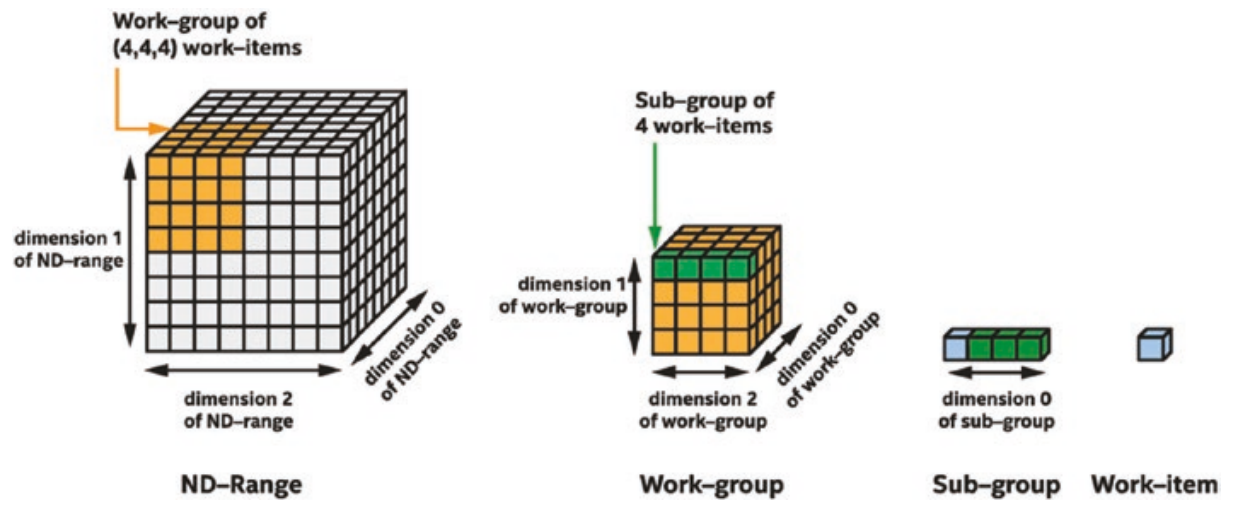
\includegraphics[width=\linewidth]{images/nd_range.png}
	\caption{Dissection of an NDRange. \textit{From Data Parallel C++} \cite{Reinders:2023:Data}.}
	\label{fig:ndrange}
\end{figure}

This coarse-grained structure enables the application of various strategies within the index space, allowing for the implementation of work-group oriented algorithm designs.
These include strategies like memory tiling, which take advantage of work-group synchronization procedures.

% ---------------------------------------------------
%
% Trabajo de Fin de Grado. 
% Author: Adriano dos Santos Moreira <alu0101436784@ull.edu.es>
% Chapter: Benchmark Comparisons
% File: Cap4_Benchmark_Comparisons.tex
%
% ----------------------------------------------------
%

\chapter{Benchmark Comparisons} \label{chap:Benchmark_Comparisons} 

In this chapter, we will run and compare various benchmarks using SYCL, CUDA and sequential CPU executions.
For this purpose, we will use \textit{HeCBench}\footnote{\href{https://github.com/zjin-lcf/HeCBench/}{{HeCBench} \url{https://github.com/zjin-lcf/HeCBench/}}}, an assortment of benchmarks specialised in heterogeneous computation.
HecBench offers over 400 different benchmarks written in HIP, OpenMP, CUDA and SYCL.

The objective of this study is to examine the practical differences between SYCL, CUDA, and serial executions in terms of performance.
Consequently, we will only provide a brief description of the algorithms and concepts used in this chapter.
For the benchmarks presented we will not go into the details of the SYCL parallelisation of the code. 
For details of the code in both CUDA and SYCL, the interested reader is referred to the source code available in the HeCBench repository for these algorithms.
In Chapter \ref{chap:CaseStudy}  we will present computational results accompanied by a comparison of SYCL and CUDA implementations for other algorithms.

Since this work serves as an introduction to heterogeneous computation and we aim to present a simplified benchmark report, we will only experiment with problem sizes in order to execute the benchmarks, with the rest of the parameters remaining at their default values.

Lastly, the graphs created for these benchmarks were plotted using Python and MatplotLib\footnote{\href{https://matplotlib.org}{{MatplotLib} \url{https://matplotlib.org}}} among other Python utilities.

\section{Execution Platform}
The experiments shown in this chapter have been executed on the \textit{Verode} platform, a computing infrastructure belonging to the High Performance Computing Group (\textit{Grupo de Computación de Altas Prestaciones} or \textit{GCAP})\footnote{\href{https://portalciencia.ull.es/grupos/6369/detalle}{{ULL GCAP} \url{https://portalciencia.ull.es/grupos/6369/detalle}}} of the Universidad de La Laguna.

\textit{Verode} is equipped with two Intel® Xeon® CPU Gold 6230N processors,  with 20 cores each, for a total of 40 cores using shared memory, this platform also provides an NVIDIA Tesla V100 GPU, especially designed for HPC and data science purposes.

Regarding the software specifications:
\begin{itemize}
    \item \textit{Verode} runs under the Debian GNU/Linux 11 (bullseye) operating system.
    \item SYCL programs were compiled using:
    \begin{itemize}
        \item \texttt{clang++} version 18.0.0.
        \item \texttt{gcc} version 12.3.0 for the GCC toolchain.
    \end{itemize}
    \item CUDA programs were compiled using:
        \begin{itemize}
            \item \texttt{nvcc} version 12.0.
            \item \texttt{gcc} version 6.5.0 as the host compiler.
        \end{itemize}
\end{itemize}

\section{Mandelbrot set}
The Mandelbrot set is a mathematical concept that was first described by Benoit Mandelbrot in 1980.
It is an infinite and infinitely complex fractal shape that emerges from a simple equation involving complex numbers.

For this specific benchmark, we had to make a small change in the code to be able to modify the size of the Mandelbrot set region.
As a result, this benchmark offers two parameters to experiment with:
\begin{itemize}
    \item \texttt{repeat}: How many times the algorithm is repeated, then averaged over all times. Using a fixed amount of 1000.
    \item \texttt{size}: Side length of the Mandelbrot set region. It always calculates a square area. Using sizes from 1000 to 45000.
\end{itemize}

Figure \ref{fig:mandelbrot-benchmark-all} shows the results for SYCL, CUDA and serial executions.

\begin{figure}[H]
	\centering
	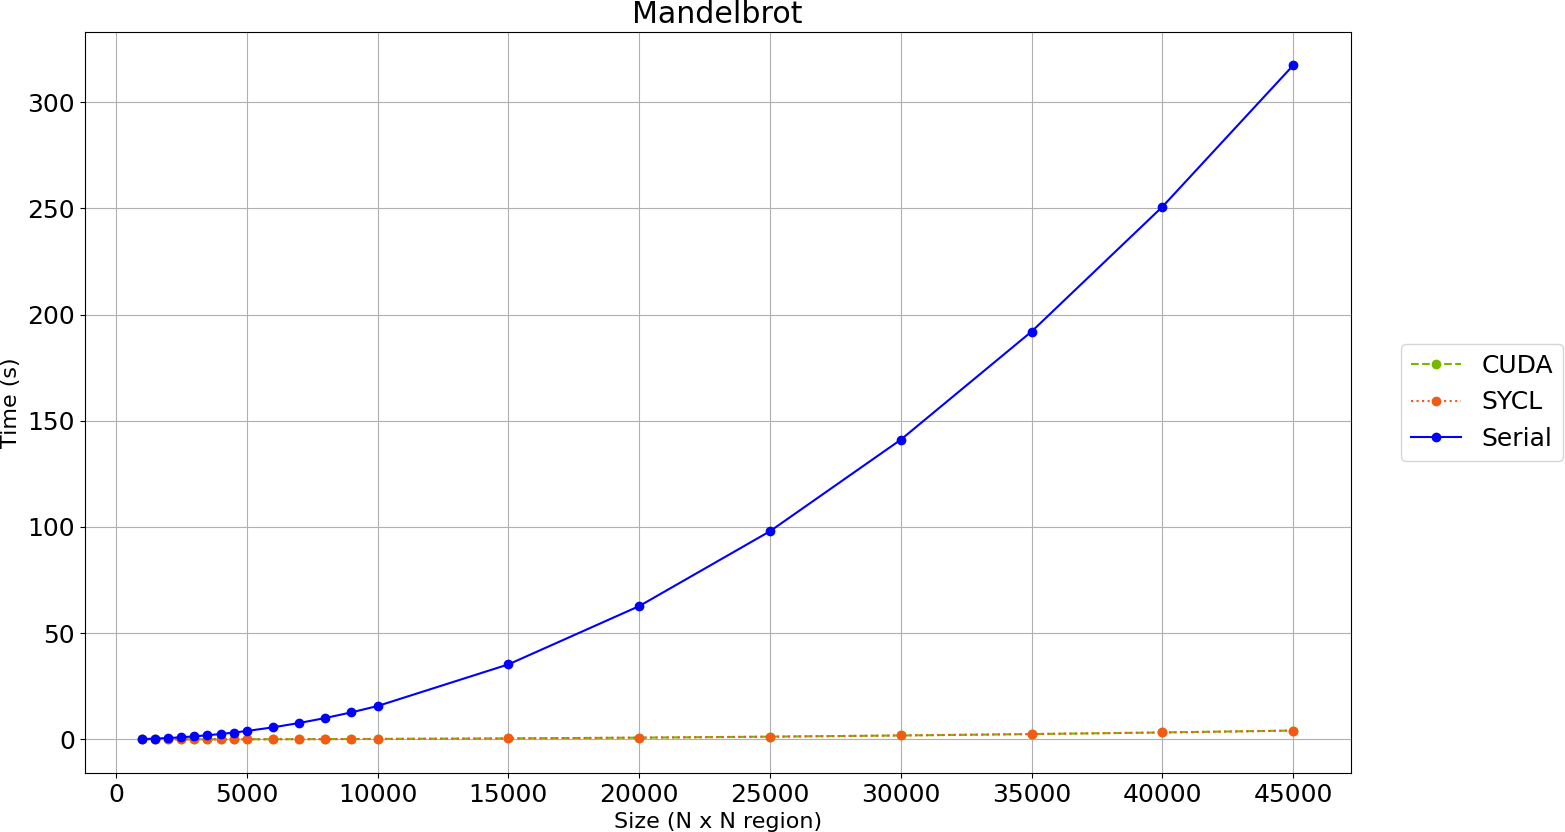
\includegraphics[width=\linewidth]{images/mandelbrot-sycl-cuda-serial.png}
	\caption{Mandelbrot benchmark. Results for SYCL, CUDA and serial executions.}
	\label{fig:mandelbrot-benchmark-all}
\end{figure}

Naturally, we can see in Figure \ref{fig:mandelbrot-benchmark-all} that CUDA and SYCL times are significantly better than serial times, reaching a gigantic time gap of over 300 seconds at size 45000.

On the other hand, in Figure \ref{fig:mandelbrot-benchmark-parallel} we can barely notice any differences when comparing the execution times of SYCL and CUDA, which speaks in favour of SYCL since it offers a higher abstraction and justifies any potential performance loss.

\begin{figure}[H]
	\centering
	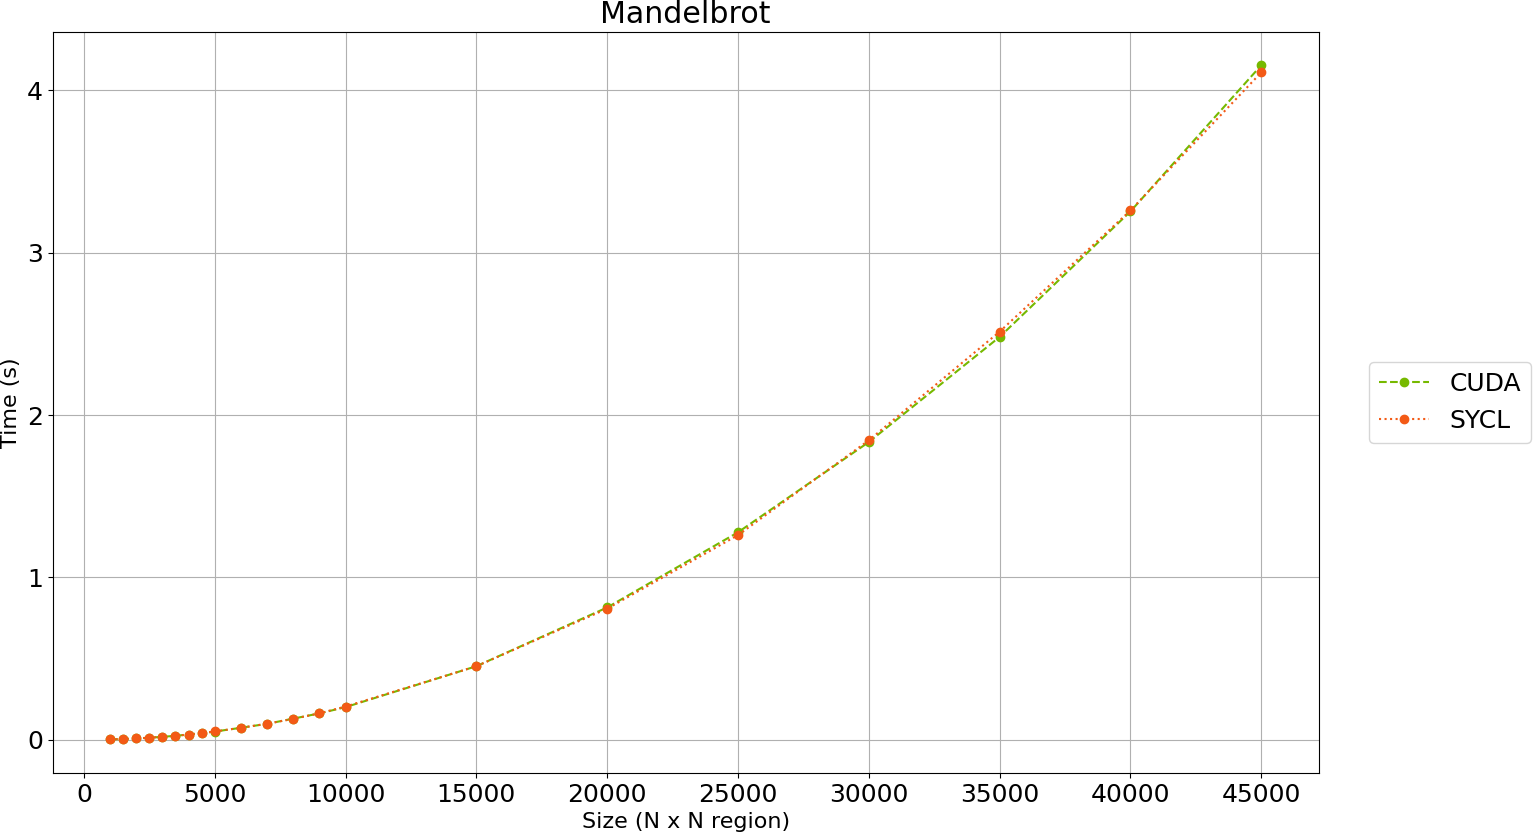
\includegraphics[width=\linewidth]{images/mandelbrot-sycl-cuda.png}
	\caption{Mandelbrot benchmark. Results for SYCL and CUDA executions.}
	\label{fig:mandelbrot-benchmark-parallel}
\end{figure}

In Figure \ref{fig:mandelbrot-speed-up}, it is observed that the speed up achieved decreases slightly as the size of the problem increases.
Again, we can see that both SYCL and CUDA results are fairly similar, although they seem to fluctuate a little.

\begin{figure}[H]
	\centering
	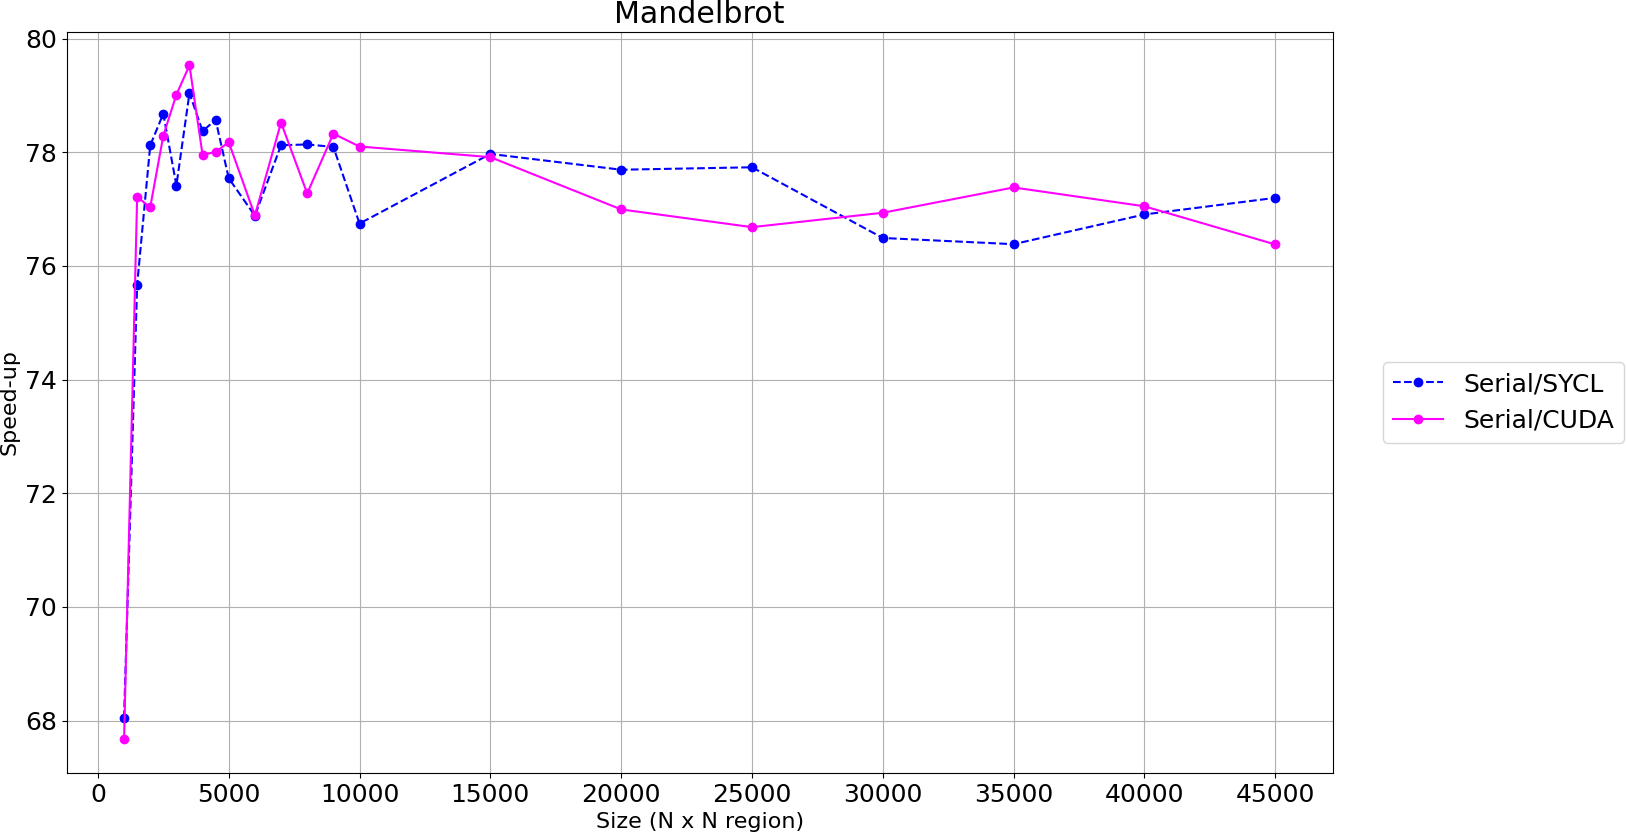
\includegraphics[width=\linewidth]{images/mandelbrot-speed-up-sycl-cuda.png}
	\caption{Mandelbrot benchmark. Speed-up graph for SYCL and CUDA executions.}
	\label{fig:mandelbrot-speed-up}
\end{figure}

\section{Floyd–Warshall algorithm}

The Floyd-Warshall algorithm is a method used to find the shortest paths in a weighted graph, where the weight of each edge represents the distance between two vertices.
Unlike other shortest path algorithms like Dijkstra's algorithm, Floyd-Warshall works for graphs with negative edge weights, as long as there are no negative cycles.

These are the parameters we can work with:
\begin{itemize}
    \item \texttt{iterations}: How many times the algorithm is repeated, then averaged over all times. Using a fixed amount of 100.
    \item \texttt{block size}: Block size used in the NDRange. Using a fixed amount of 16.
    \item \texttt{number of nodes}: Amount of nodes in the weighted graph. Using 500 to 10000 nodes.
\end{itemize}

Figure \ref{fig:floydwarshall-benchmark-all} presents the resulting graph for SYCL, CUDA and serial executions.

\begin{figure}[H]
	\centering
	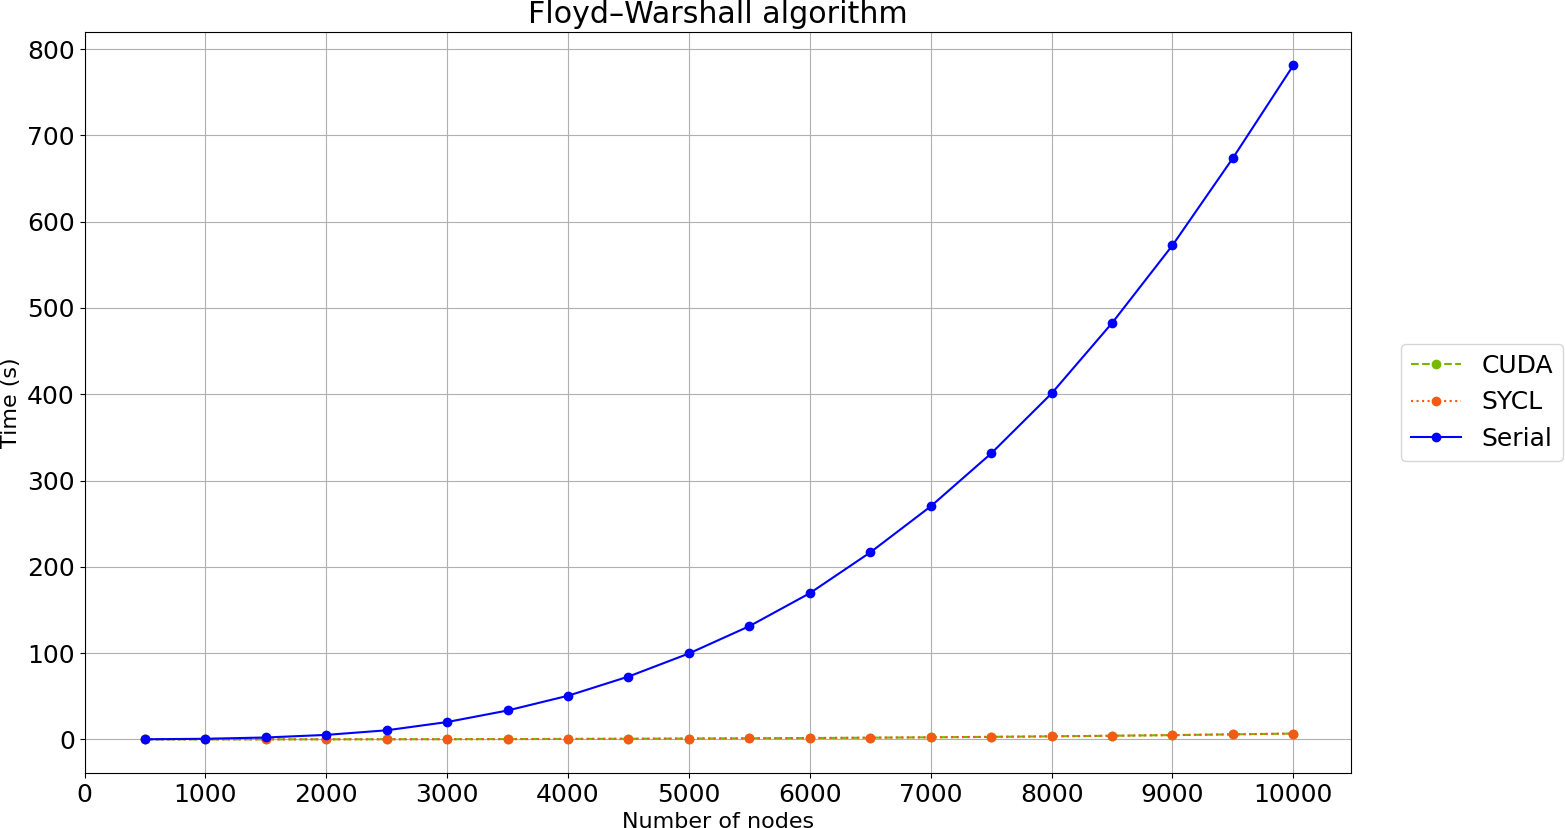
\includegraphics[width=\linewidth]{images/floydwarshall-sycl-cuda-serial.png}
	\caption{Floyd–Warshall algorithm. Results for SYCL, CUDA and serial executions.}
	\label{fig:floydwarshall-benchmark-all}
\end{figure}

The resulting graph in Figure \ref{fig:floydwarshall-benchmark-all} clearly demonstrates that serial execution is significantly slower than both SYCL and CUDA implementations as the problem size increases.

A closer examination of SYCL and CUDA graphs (Figure \ref{fig:floydwarshall-benchmark-parallel}) reveals that most execution instances exhibit a high degree of similarity in terms of execution time.
However, the last three problem sizes show the greatest differences, although these are not too significant.

\begin{figure}[H]
	\centering
	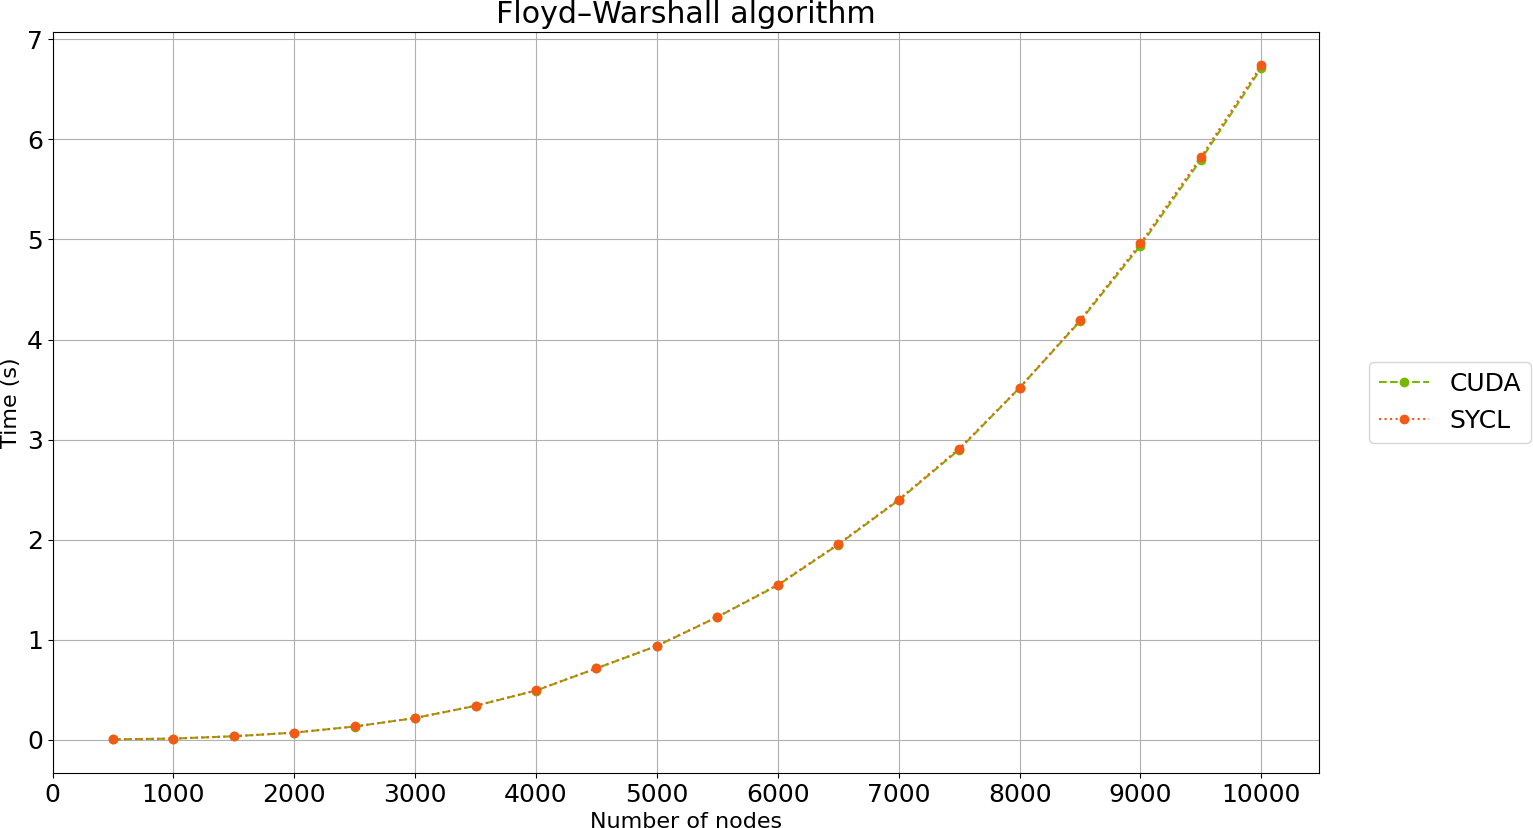
\includegraphics[width=\linewidth]{images/floydwarshall-sycl-cuda.png}
	\caption{Floyd–Warshall algorithm benchmark graph for SYCL and CUDA executions.}
	\label{fig:floydwarshall-benchmark-parallel}
\end{figure}

In terms of speed-up, Figure \ref{fig:floydwarshall-speed-up} reflects an almost identical graph for SYCL and CUDA, tracing a logarithmic-like representation in both cases.

\begin{figure}[H]
	\centering
	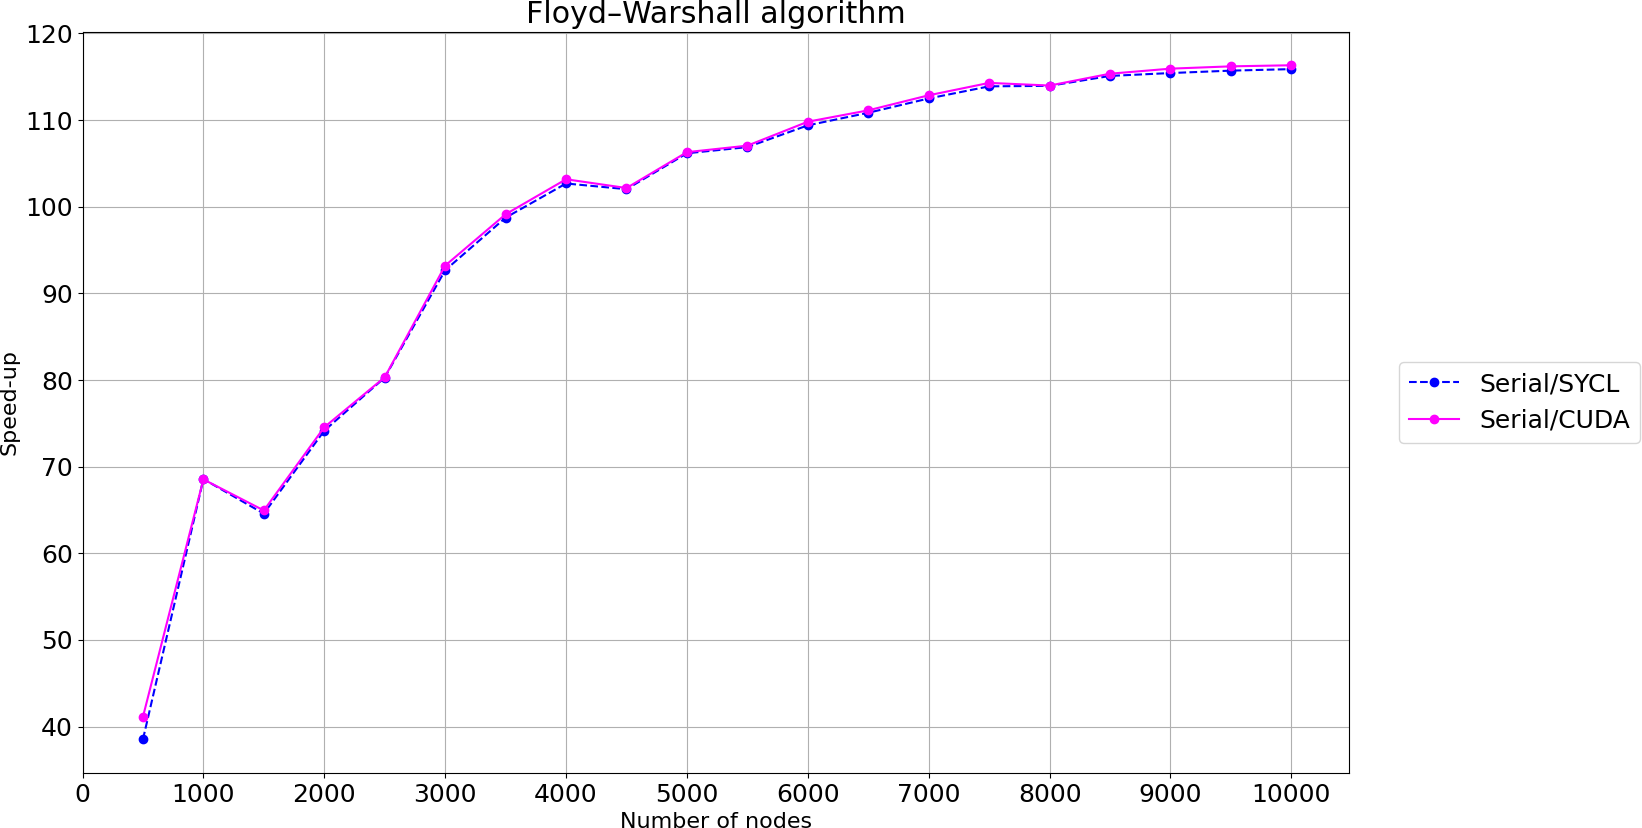
\includegraphics[width=\linewidth]{images/floydwarshall-speed-up-sycl-cuda.png}
	\caption{Floyd–Warshall algorithm speed-up graph for SYCL and CUDA executions.}
	\label{fig:floydwarshall-speed-up}
\end{figure}

\section{Molecular dynamics}
Molecular dynamics (MD) is a powerful computational simulation technique used to study the physical movements of atoms and molecules over time.
By applying the principles of classical mechanics, MD allows scientists to predict the behavior of matter at the molecular level, offering insights into the structural, dynamic, and thermodynamic properties of complex systems such as proteins, nucleic acids, and materials.

Once more, the original benchmark had to be slightly modified to be able to input different problem sizes.
There are two parameters we can work with:
\begin{itemize}
    \item \texttt{problem size}: Number of atoms in the simulation. Using sizes 2500 to 1000000.
    \item \texttt{iterations}: How many times the MD kernel is executed, then averaged over all times. Using a fixed amount of 1000.
\end{itemize}

\begin{figure}[H]
	\centering
	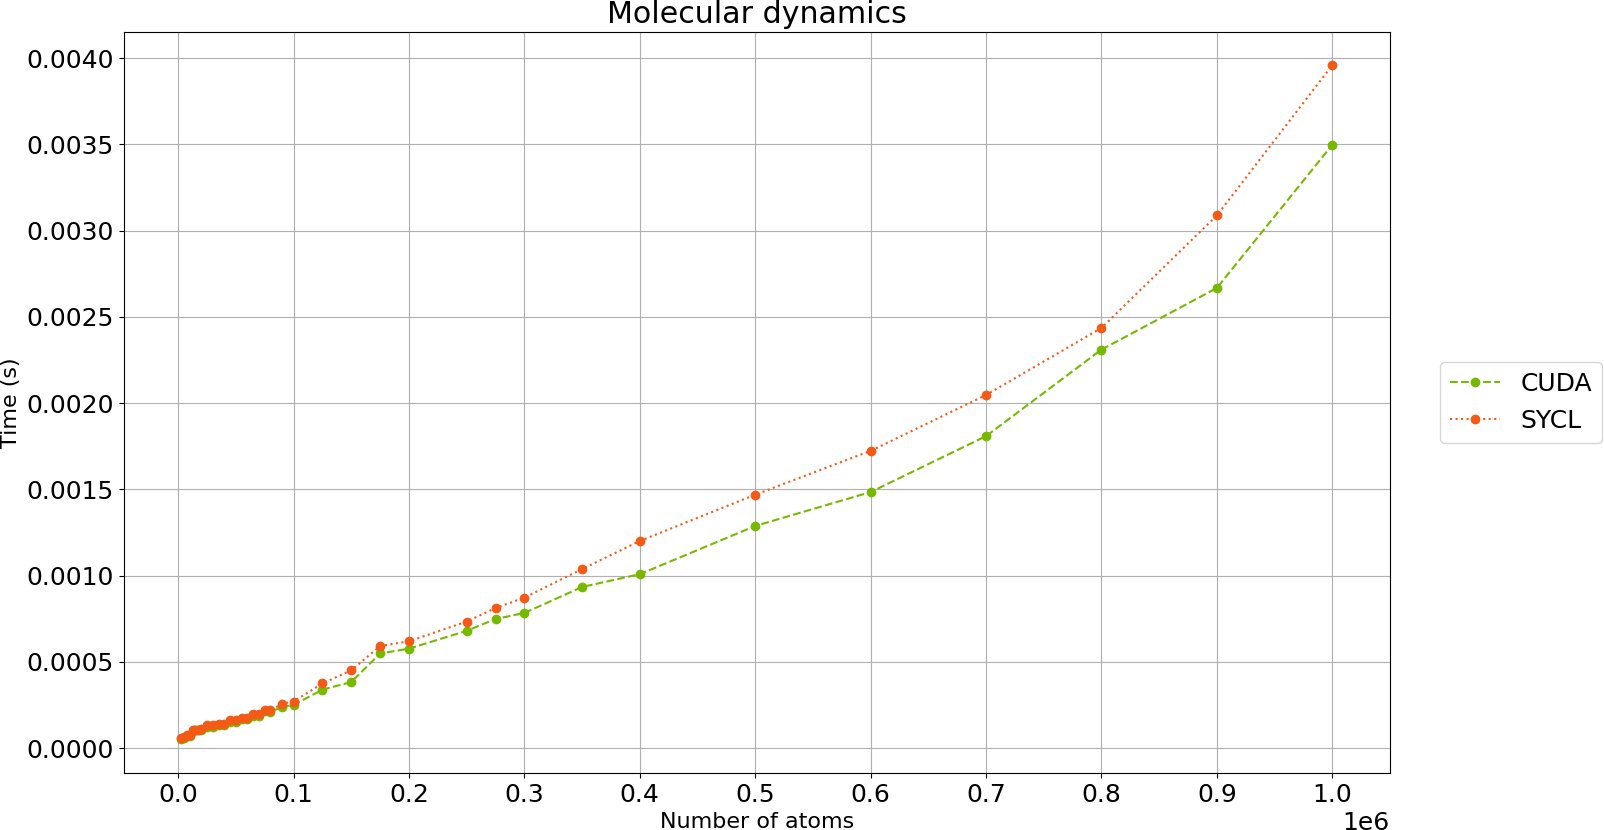
\includegraphics[width=\linewidth]{images/md-sycl-cuda.png}
	\caption{MD benchmark. Results for SYCL and CUDA executions.}
	\label{fig:md-sycl-cuda}
\end{figure}

In Figure \ref{fig:md-sycl-cuda} we measured the average kernel execution time for each selected size.
From this graph we can see that both implementations run at similar speeds, although CUDA becomes up to 11.65\% faster (on problem size 1000000) than SYCL as the number of atoms increases.

\section{Backpropagation}
Backpropagation, is a fundamental algorithm in machine learning, particularly in the training of artificial neural networks.
It enables the development of complex models that can perform tasks such as image recognition and natural language processing.
The algorithm works by iteratively adjusting the weights of the network to minimize the difference between the predicted output and the actual target output, which is measured by a loss function.

In this case, the algorithm has a single parameter: the \texttt{number of input nodes} (number of nodes in the neural network). The code requires a value divisible by 16 and for these experiments the value ranges from 512 to 1024000. 
What is being measured is the device offloading time for all execution instances.

\begin{figure}[H]
	\centering
	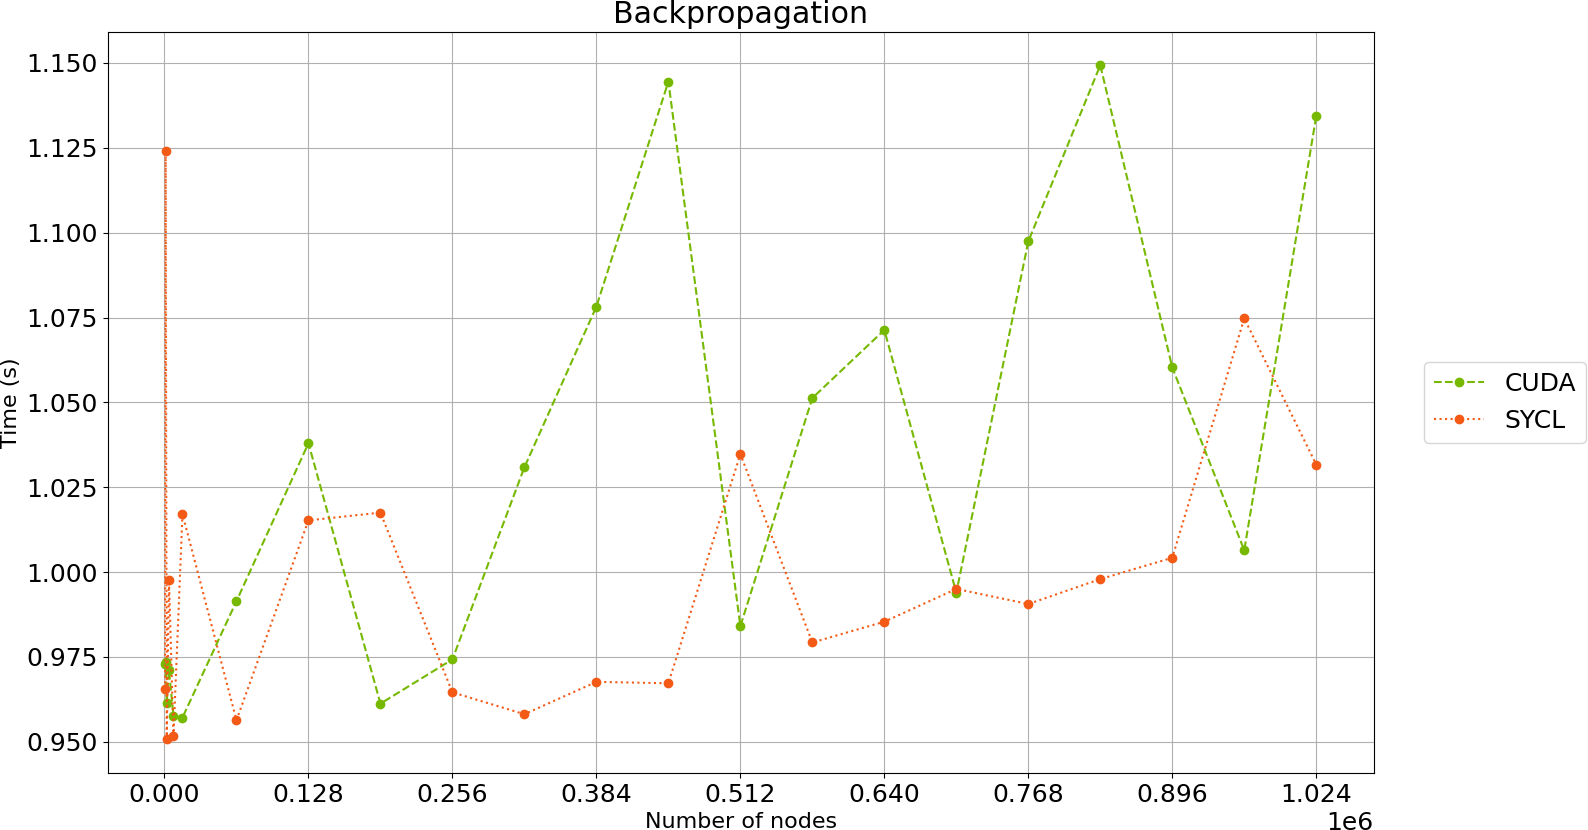
\includegraphics[width=\linewidth]{images/backprop-sycl-cuda.png}
	\caption{Backpropagation benchmark. Results for SYCL and CUDA executions.}
	\label{fig:backprop-sycl-cuda}
\end{figure}

The results in Figure \ref{fig:backprop-sycl-cuda} show a large variation in CUDA/SYCL runtimes for each problem size.
In this experiment, SYCL seems to be a bit more stable in terms of time fluctuation.

The SYCL version of this algorithm has a limitation since the maximum problem size supported is near 1.048.000 nodes, while the CUDA implementation surpasses this constraint.

\lstinputlisting[language=log,style=logstyle,caption={NDRange error on backpropagation benchmark.},label={listing:error-backprop-sycl}]{listings/error_backprop_sycl.log}

This limitation can be evidenced by using \texttt{1,048,800} as the problem size.
Listing \ref{listing:error-backprop-sycl} is the output of this experiment and line 14 shows the root of this limitation.
The problem is that the number of resulting work-groups that the program pretends to create exceeds the maximum established by the compiler.

This constraint is not tied to the SYCL specification but the compiler implementation, which is \texttt{clang++} in this case.
Since the hardware is always a physical and tangible limit, this particular compiler has decided to set an arbitrary limit for this very reason.

One solution to this situation would be to assign more work to each work-group.
This would reduce the number of work-groups so that it does not hit the limit set by the compiler.



% ---------------------------------------------------
%
% Trabajo de Fin de Grado. 
% Author: Adriano dos Santos Moreira
% Chapter: Full SYCL Implementation
% File: Cap5_Full_SYCL_Implementation.tex
%
% ----------------------------------------------------
%

\chapter{An Industry Case Study: Image Processing with SYCL} \label{chap:CaseStudy} 

In this chapter we will take a deep look into the development of a SYCL application.
For this purpose, we have contacted Wooptix\footnote{\url{https://wooptix.com}}, a Canary Islands based company with expertise in image processing.
To illustrate their needs, Wooptix suggested the implementation of the erosion operation on FITS format images and they provided us with one of the images they use for real purposes.

The erosion is one of the fundamental operations in morphological image processing \cite{Gonzalez:2008:Digital}.
This branch of knowledge studies the structure and components of an image with the objective of creating useful descriptions of its shape, while also providing tools for signal processing.

On the other hand, the FITS (Flexible Image Transport System) file format is the standard astronomical data format supported by NASA and the IAU (International Astronomical Union).
This standard supports multi-dimensional images, although we will only focus on two-dimensional FITS files.

The application presented in this chapter was developed using C++.
To open and process images in FITS format, we will use CFITSIO\footnote{\href{https://heasarc.gsfc.nasa.gov/fitsio/}{{FITSIO Home Page} \url{https://heasarc.gsfc.nasa.gov/fitsio/}}}, a library of C and Fortran subroutines for reading and writing FITS files.

\section{The erosion operation}

The erosion operation is used to shrink or erode the boundaries of objects within an image applying a structuring element.

\vspace{5mm}
\textsl{\textbf{{Structuring Element}}}
\vspace{2mm}

A structuring element (SE) is a mask which determines how the operation is applied to the image.
This object is usually represented by a matrix, where non-zero values describe the mask and a center origin to apply the mask from.
We can classify them in two types:
\begin{itemize}
    \item \textbf{Flat SE}: Composed of 0s and 1s only, simply establishes which pixels are relevant and which are not.
    \item \textbf{Non-flat SE}: Contains grayscale values that describe how meaningful the pixels are.
\end{itemize}

For this application, we will work with two-dimensional grayscale images using flat structuring elements.

The erosion operation consists of sliding a SE over an entire image, applying the SE to each pixel.
This procedure takes the lowest value in the vicinity established by the SE (with a value of 1) and assigns it to the evaluated pixel, creating an output image whose bright regions are shrunk and dark regions are enlarged.

\begin{figure}[H]
    \centering
    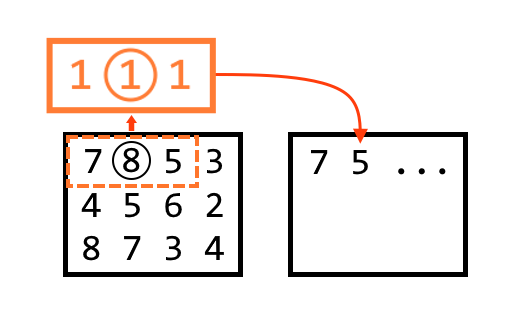
\includegraphics[width=0.5\linewidth]{images/erosion_graph.png}
    \caption{Simplified erosion operation.}
    \label{fig:erosion-graph}
\end{figure}

In Figure \ref{fig:erosion-graph} we can see a graphical example of this transformation.
In this illustration, the second element of the input image is evaluated.
According to the SE, the neighborhood of the element is 7, 8 and 5, from which we can conclude that the lowest value is 5, resulting in the value of erosion at the second pixel.

Note that certain border regions of the image make the SE go out of bounds.
In order to process image borders correctly, we add padding around the image with a very high value, ensuring that the algorithm only considers pixels within the original image.
\pagebreak
\section{Supporting Code}

In order to implement the erosion operation, we need to create an environment to work on images in FITS format, as well as to represent the structuring element and make everything work together.

The supporting code is based on three main classes:
\begin{itemize}
    \item \texttt{FitsImage}: Encapsulates the functionality of the CFITSIO library.
    \item \texttt{StructuringElement}: Represents a SE and provides access to every detail of it.
    \item \texttt{Morphology}: Base class for the morphology operations, this makes the project easily expandable.
\end{itemize}

One important aspect to note is that the FITS format supports many pixel sizes, so the number of bytes a pixel occupies may vary from file to file.
This is important to have into account because we need to maintain format consistency when reading, operating and writing the image we work with.

Depending on the pixel size, the application will decide on a data type in runtime, which can be one of the following: \texttt{unsigned char}, \texttt{short}, \texttt{long}, \texttt{long long}, \texttt{float} or \texttt{double}.

Because we are using C++, we need to use polymorphism in combination with the factory method pattern\footnote{\href{https://refactoring.guru/design-patterns/factory-method}{{Factory method} \url{https://refactoring.guru/design-patterns/factory-method}}} to achieve dynamic type behaviour in our program.

\begin{figure}[H]
    \centering
    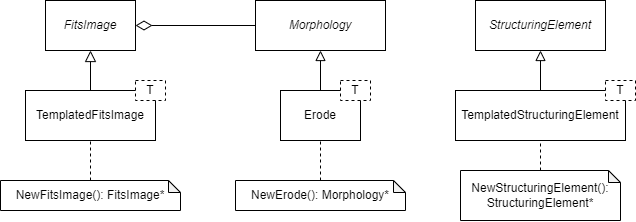
\includegraphics[width=0.85\linewidth]{images/morph_uml.png}
    \caption{Conceptual UML class diagram for the erosion application.}
    \label{fig:uml-morph-graph}
\end{figure}

This dynamic typing was made possible thanks to the implementation of the abstract base classes described in Figure \ref{fig:uml-morph-graph}.
Each of these classes derive in a class template that can be used to dynamically create instances by using a non-member function, also indicated in the diagram with a note for every concrete class.

\section{Erosion Solution Development}

We present two implementations for the erosion operations, this section is dedicated to explain in detail how the operation is performed in both serial and SYCL approaches.

It would be beneficial to keep a few notes in mind when reading the implementations:
\begin{itemize}
    \item Both \texttt{FitsImage} and \texttt{StructuringElement} data are stored in generic type one-dimensional arrays.
    \item Data arrays are stored in row-major order, starting from the bottom left.
    \item The code shown operates directly on the image representation, modifying the \texttt{FitsImage} content.
\end{itemize}

\subsection{Serial Implementation}

The serial implementation of the erosion operation presented here is quite straightforward.
This approach provides a baseline against which the performance of the parallel version can be measured, while also serving as a reference to see whether its parallel version is worth the effort.

In addition, writing a naive implementation can provide insight into the complexity and potential bottlenecks of the algorithm, and help understand how the algorithm scales with increasing data or computational load.

The algorithm can be divided in two main zones.
The first is the preparation for the erosion and the second is the erosion itself.
\pagebreak

\lstinputlisting[language=C++,style=cppstyle,caption={Serial erosion function. \href{{https://github.com/AdrianoMoreira08/TFG-SYCL/blob/main/image-processing/morphology-gray/include/erode.h}}{\textit{See on Github}}.},label={listing:serial-morph-full}]{listings/serial_morph_full.cc}

The first action of the preparation code is to cast both the FITS image and the structuring element pointers into their corresponding concrete class, which have the accessors to the template dependant arrays of data.
This happens in lines 2-5.
Then, lines 6 and 9 retrieve both image and SE data pointers.

We cannot read and write over the same image data, since it would modify the neighbourhood of pixels we will operate on later.
To avoid this situation, we create a copy of the image data in line 8.

To conclude the set-up, we calculate the location of the first pixel of the image in line 10.

The erosion operation itself starts from line 11, where the main loops (lines 11 and 13), traverse the whole image.
After every row, we calculate the first index of said row for the image data array in line 12, and for every column, we obtain the pixel index in line 14 for the pixel we will evaluate.
Another relevant index is the location of the first pixel that corresponds to the SE evaluation, calculated in lines 15-17.

The region of code that covers lines 18-30 determines the output pixel value of the current pixel, which calculates the minimum pixel value in the neighbourhood set by the SE.

Starting in line 18, we set a very high minimum value for the output pixel.
Then, the loops in lines 19 and 22 traverse the whole structuring element.
For every row, we calculate the first index of said row for the image data array as well as for the SE, accomplished in lines 20-21.

In the innermost loop, we compute the neighbour pixel index to be evaluated in line 23 and check if the structuring element considers that pixel and whether its value is the new minimum.
If it passes the checks, the new minimum is assigned in line 26.
After the calculation of the minimum, it is set as the new pixel value in line 30.
As a last action, we delete the copy of the image in line 33.

\subsection{SYCL Implementation}

The parallel implementation using SYCL is based on the naive algorithm presented in the serial implementation.
Nevertheless, a parallel approach to this algorithm is clear to give significant benefits if we take into account the embarrassingly parallel nature of it.
To be more specific, the fact that each pixel of the image is processed independently of each other, makes it an ideal candidate for parallel execution.
Moreover, if we implement memory tiling to this process, the the efficiency can be further enhanced.

Memory tiling involves dividing the image into smaller blocks that fit into the fast, local memory dedicated to every work-group.
By doing so, we can significantly reduce the latency associated with accessing global memory.
Each tile can be loaded into the local memory, processed independently, and then the results can be written back to global memory.
This approach minimizes memory access delays and improves data locality, ensuring that each work-item spends more time computing and less time waiting for data.

For this implementation we will use the buffer/accessor model, covered in Section \ref{sec:buffer-accessor} of Chapter \ref{chap:SYCL}.
\pagebreak

\lstinputlisting[language=C++,style=cppstyle,caption={Set-up for SYCL parallel execution. \href{{https://github.com/AdrianoMoreira08/TFG-SYCL/blob/main/image-processing/morphology-gray/include/erode_sycl.h}}{\textit{See on Github}}.},label={listing:sycl-morph-setup}]{listings/sycl_morph_setup.cc}

In Listing \ref{listing:sycl-morph-setup} we have the preparation code for the kernel execution.
Firstly, we create a queue and select a GPU device in line 1.
Then we retrieve both image and SE pointers and their data (lines 2-7), the same way we did for the serial version.

Lines 9-13 set padding related ranges and offsets.
Line 15 starts the buffer scope, outside of which the buffers are destroyed.

Following, we have two sets of ranges.

In the first one, line 17 specifies the size of the work-groups of the NDRange, which is defined to be the same size as the SE.
Then we define how many work-groups we need by dividing the image dimensions by the local range and taking the ceiling of the result.
This is calculated in lines 18-21.
After this, we can calculate the global range and set the NDRange in lines 22-24.

The second set of ranges calculates buffer sizes.
Both input and output image buffer ranges are the same size (lines 26-29) and is set to the size of the original padded image.
The SE range, in line 30 has the same dimensions as the SE itself.
On the other hand, in line 31, the tile range is set to be the local range plus twice the padding, ensuring that the structuring element does not to surpass the tile range.

The next 33-37 lines simply create the buffers using the previously defined ranges and data pointers.
Note that line 34 indicates that the image buffer has nowhere to write back when the buffer is destroyed, this is specified to ensure that there is no time lost writing unnecessary data back.
On the other hand, line 36 gives the output buffer a pointer to write back to, which is the pointer to the original data array, successfully overwriting the data.
\pagebreak
\lstinputlisting[language=C++,style=cppstyle,firstnumber=38,caption={Erosion operation kernel using SYCL. \href{{https://github.com/AdrianoMoreira08/TFG-SYCL/blob/main/image-processing/morphology-gray/include/erode_sycl.h}}{\textit{See on Github}}.},label={listing:sycl-morph-operation}]{listings/sycl_morph_operation.cc}

The erosion operation occurs in Listing \ref{listing:sycl-morph-operation}, where we submit the command group to the queue (line 39).
Just before the kernel starts, we define a series of accessors in lines 40-42, which correspond to the image (read-only), output (write-only) and SE (read-only).
A fourth accessor is present in line 43, which grants access to the local memory to perform the memory tiling with.

Line 45 starts the definition of the kernel.
First, we set various indexes related to the current work-item (lines 46-49):
\begin{itemize}
    \item \textbf{Global ID}: Unique global identifier.
    It matches with the output pixel index since the \texttt{parallel\_for} range coincides with the image range.
    \item \textbf{Group ID}: Identifies the work-group.
    Useful to calculate where the work-group tile begins within the image.
    \item \textbf{Local ID}: Index of the work-item within the work-group.
    Determines which pixels the work-item has to copy to the tile and the offset to read within the tile.
    \item \textbf{Global group offset}: First index of the tile within the image.
\end{itemize}

In order to write the whole tile, each work-item of the work-group contributes to copy from the image to the tile without repeating.
This is done in lines 52-56, where each work-item starts at a unique position determined by the local ID and iterates in increments of the size of the local range.
This approach ensures that no work item repeats the copy operation on the same pixel.

To guarantee that every work-item has access to the same exact full information of the tile, line 57 sets a group barrier which makes all work-items in the work-group wait until each one has reached this point in the code.
Right after, we calculate the starting point where the SE will be applied within the image.
Line 58 determines this starting point, obtaining the index of the first element to be read, which will serve as an offset in the next calculations.

The computation for the new pixel value starts by setting a very high number as the new minimum in line 61.
Following, we iterate over the SE using loops 62 and 63.
In the innermost loop, we start by identifying which pixel of the image to analyze in line 64.
Then, if the current position of the SE indicates that such pixel may be considered, we evaluate whether the pixel value is the new minimum.
This process happens in lines 65-68.
The new minimum value is written in the output buffer in line 72.

Finally, we wait in line 75 for this task to finish.
\pagebreak

\section{Results}

In this section, we will present the application of the erosion operation on various images.
We will also display the global compute time of each program as well as the isolated time for the operation only.
The code presented in the previous section was run on \textit{Verode}, the same platform described in Chapter \ref{chap:Benchmark_Comparisons}.

The first image we will process was created using the the Faint Object Camera (FOC) from the Hubble Space Telescope in July 1996, with the size of 1024 by 1024 pixels.
This picture is part of a sample collection\footnote{\href{https://fits.gsfc.nasa.gov/fits\_samples.html}{{Sample FITS Files} \url{https://fits.gsfc.nasa.gov/fits\_samples.html}}} listed by NASA.
In Figure \ref{fig:og-foc} we can see this image.

\begin{figure}[H]
    \centering
    \includegraphics[width=0.5\linewidth]{images/og-foc.png}
    \caption{Original FOC sample image.}
    \label{fig:og-foc}
\end{figure}

For this first experimentation, we will use the structuring element shown in Listing \ref{listing:cross-se}. 
It defines a simple cross shape whose chosen center is (1, 1), the second element of the second row.

\begin{tabular}{c}
\lstinputlisting[language=C++,style=cppstyle,caption={Cross-shaped structuring element.},label={listing:cross-se}]{listings/cross.txt}
\end{tabular}

Figure \ref{fig:result-foc} illustrates a magnified comparison of the original (left) and eroded (right) images.
Given that both serial and SYCL implementations yield the same final image, there is no need to display or differentiate the resulting images.

\begin{figure}[H]
    \centering
    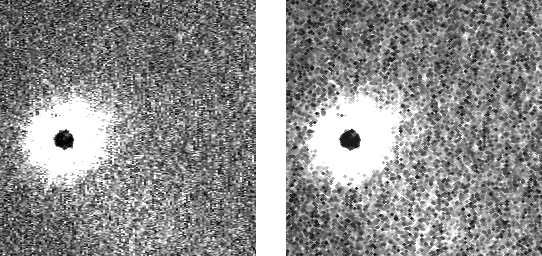
\includegraphics[width=0.7\linewidth]{images/FOC-result.png}
    \caption{Zoomed in FOC image. Original (left) and eroded (right).}
    \label{fig:result-foc}
\end{figure}

Executing both serial and parallel versions 10 times and averaging the times, we find the following results:

\begin{itemize}
    \item The overall program execution time is 1.10 seconds for serial and 1.30 seconds for SYCL.
    \item The operation execution time is 0.04 seconds for serial and 0.17 seconds for SYCL.
\end{itemize}

For this specific test, both overall and operation times are lower for the serial version.
This is expected since smaller images may suffer from the overhead introduced by the parallel SYCL version, while larger images would greatly benefit from the parallel implementation.

To prove that the SYCL implementation can actually outperform the serial version, we worked with a large sample image provided by Wooptix.
The image size is is 6388 by 6388 pixels and you can see it in \ref{fig:og-wooptix}.

\begin{figure}[H]
    \centering
    
\includegraphics[width=0.5\linewidth]{images/og-wooptix.png}
    \caption{Original Wooptix sample image.}
    \label{fig:og-wooptix}
\end{figure}

The following testing will be performed using a 8 by 8 circle-shaped structuring element, represented in Listing \ref{listing:circle-se}, whose chosen center is (3, 3) or the fourth element of the fourth row.

\begin{tabular}{c}
\lstinputlisting[language=C++,style=cppstyle,caption={Circle-shaped structuring element.},label={listing:circle-se}]{listings/circle.txt}
\end{tabular}

The result of the operation can be observed in Figure \ref{fig:result-wooptix}, distinguishing the original image from the eroded one.
Although it appears to be a minor change, the difference can be seen by observing the dark spot near the center of the image.

\begin{figure}[H]
    \centering
    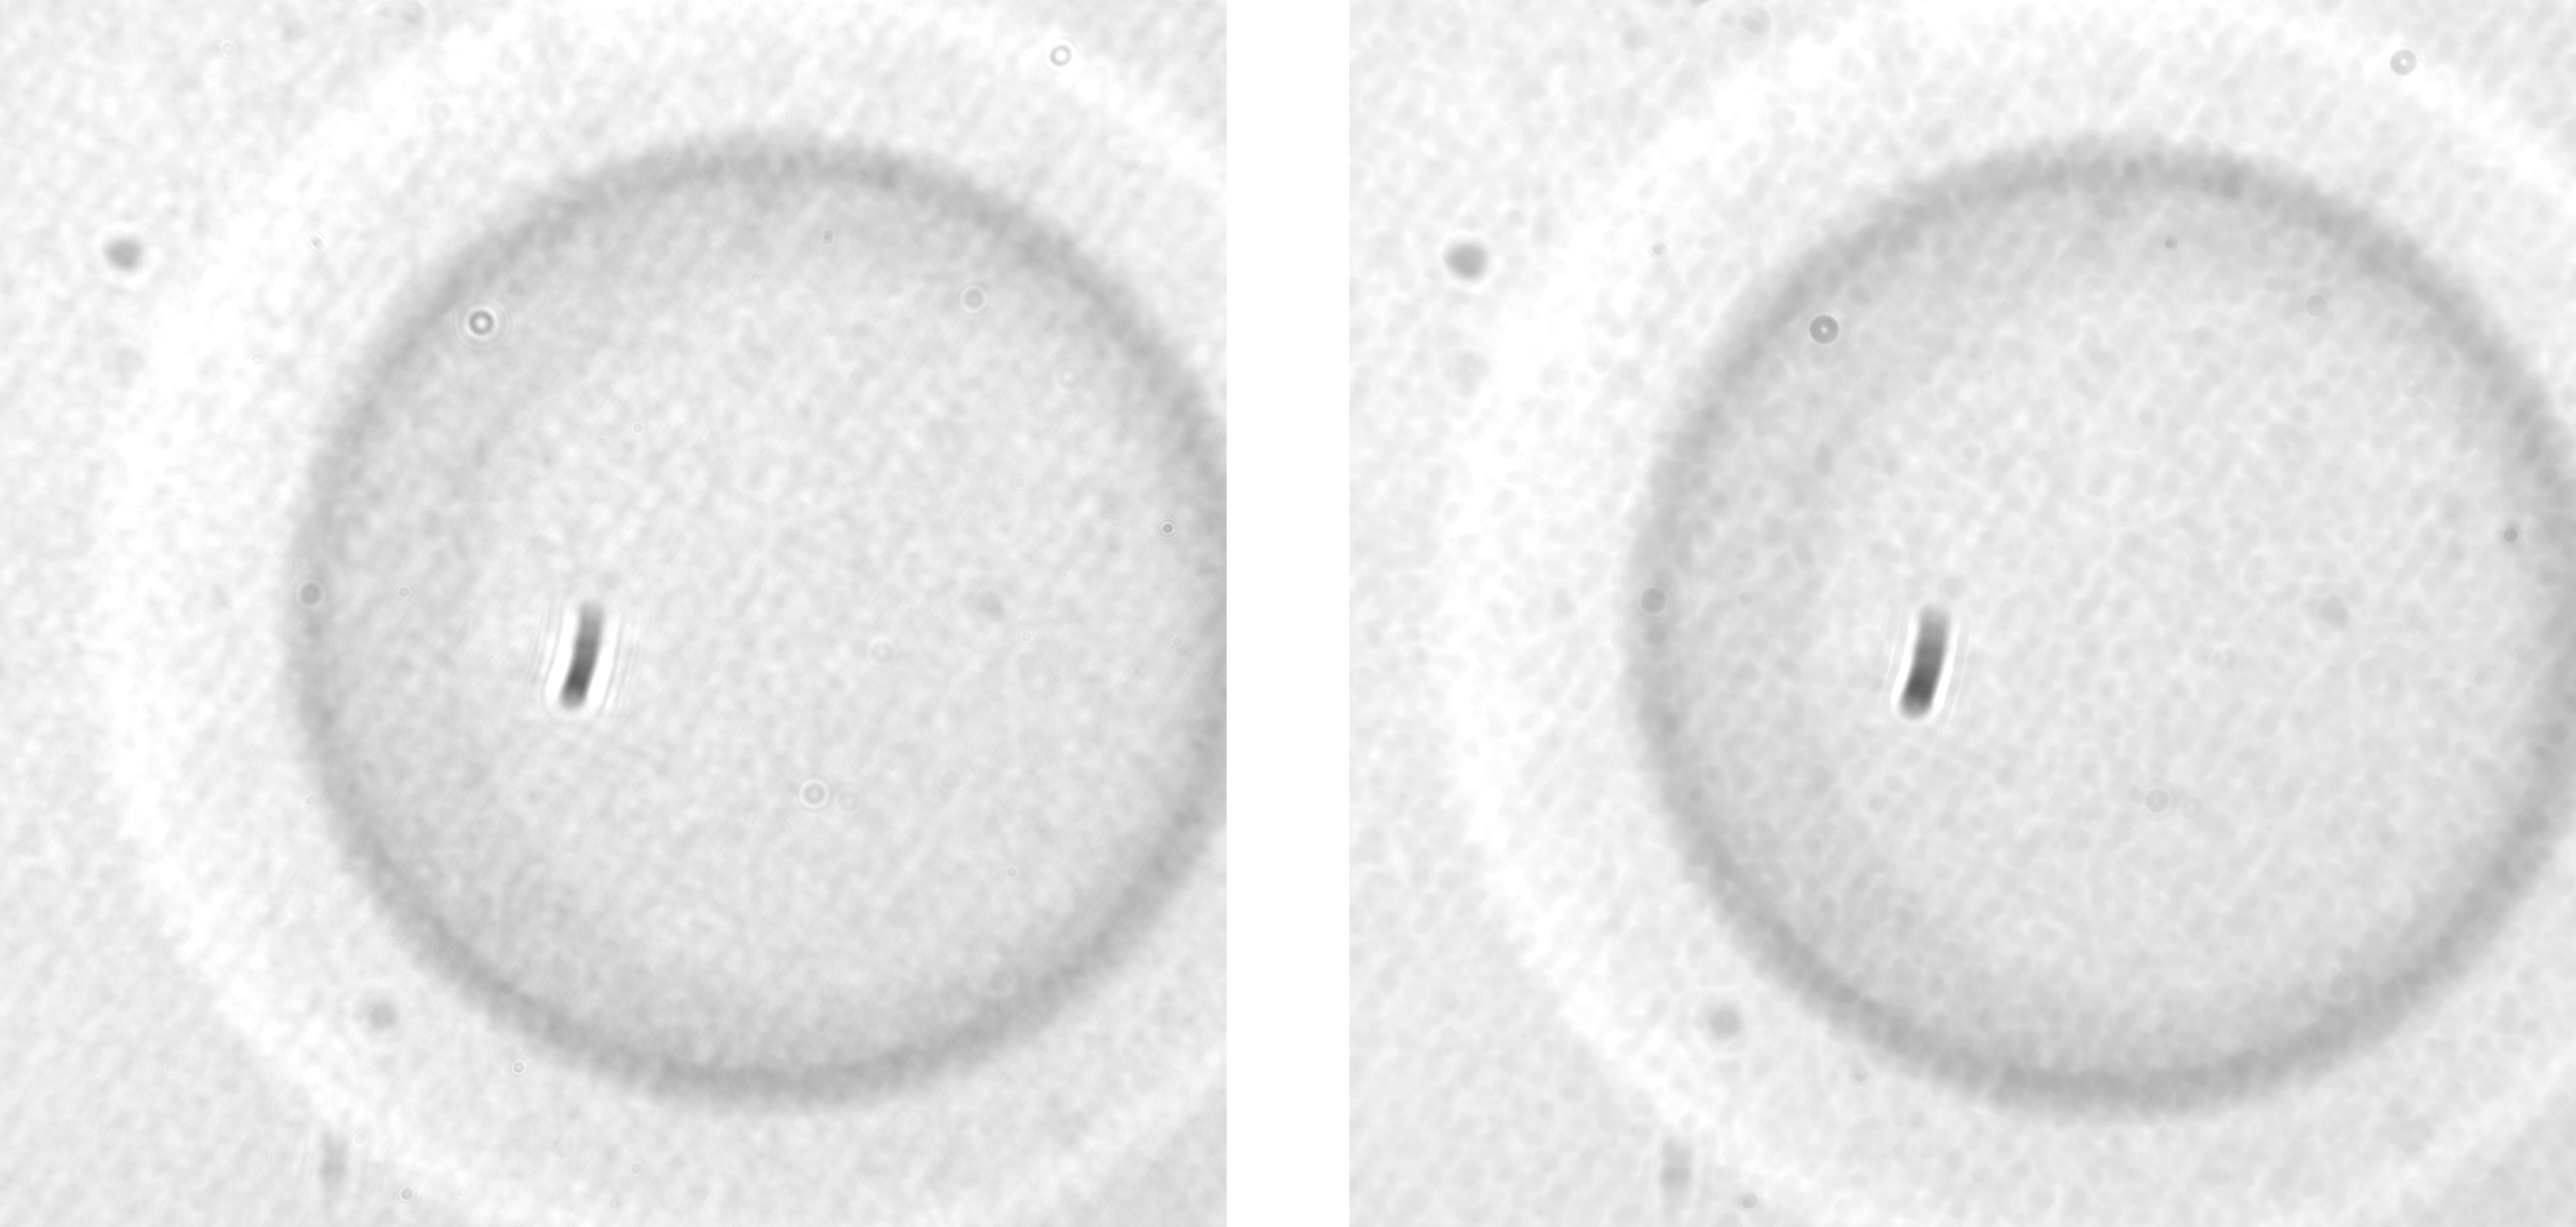
\includegraphics[width=0.7\linewidth]{images/comparison-wooptix.png}
    \caption{Zoomed in Wooptix sample image. Original (left) and eroded (right).}
    \label{fig:result-wooptix}
\end{figure}

Once again, executing the algorithm 10 times and averaging the resulting times, we can see the following differences in time:

\begin{itemize}
    \item The overall program execution time is 58.61 seconds for serial and 56.30 seconds for SYCL.
    \item The operation execution time is 3.32 seconds for serial and 0.29 seconds for SYCL.
\end{itemize}

Considering all 10 execution instances, the overall program execution time varies from 45 to 70 seconds for both serial and SYCL implementations.
On the other hand, the SYCL version clearly outperforms the serial version when it comes to the execution of the erosion operation itself, gaining a speed-up of factor 11.5.

% ---------------------------------------------------
%
% Trabajo de Fin de Grado. 
% Author: Álvaro Fontenla aluXXX@ull.edu.es
% Chapter: Conclusions and Future Lines of Work
% File: Cap6_Conclusiones_y_Lineas_de_Trabajo_Futuras.tex
%
% ----------------------------------------------------
%

\chapter{Conclusiones y Líneas de Trabajo Futuras} \label{chap:Conclusiones} 

En este capítulo se presentarán las conclusiones alcanzadas tras la realización de este trabajo y discutiremos posibles líneas futuras de trabajo.
Las conclusiones y resultados obtenidos de este proyecto de investigación y desarrollo pueden resumirse en los siguientes puntos:

\begin{itemize}
    \item Un primer valor añadido del trabajo realizado ha sido la contextualización y aprendizaje realizado por el estudiante en el ámbito de la computación de altas prestaciones. Dada la escasez de materias relacionadas con este tópico en el Grado en Ingeniería Informática en la Universidad de La Laguna, el estudiante ha tenido que realizar inicialmente un esfuerzo significativo en el aprendizaje de conceptos y técnicas que le eran ajenos.
    
Existen algunas líneas de trabajo futuras abiertas a exploración que podrían ayudar a ampliar y profundizar en los beneficios y aplicaciones de SYCL en el ámbito de la computación de altas prestaciones.
Son las siguientes:

 \begin{enumerate}
     \item Implementación y benchmarking para diferentes back-ends y/o hardware de destino empleando SYCL. Debido a las limitaciones en cuanto al hardware disponible, las únicas plataformas con las que se ha experimentado son CPU y GPU. Sería interesante extender los experimentos realizados a otras plataformas.
 \end{enumerate}




% ---------------------------------------------------
%
% Trabajo de Fin de Grado. 
% Author: Adriano dos Santos Moreira
% Chapter: Conclusions and Future Lines of Work
% File: Cap7_Conclusions_and_Future_Lines_of_Work.tex
%
% ----------------------------------------------------
%

\chapter{Conclusions and Future Lines of Work} \label{chap:Conclusions} 


This chapter will present the conclusions reached after the completion of this work and discuss possible future lines of work.
The conclusions and results obtained from this research and development project can be summarised in the following points:

\begin{itemize}
    \item A first added value of the work done has been the contextualisation and learning carried out by the student in the field of high performance computing. Given the scarcity of subjects related to this topic in the Degree in Computer Science at the Universidad of La Laguna, the student has initially had to make a significant effort in learning concepts and techniques that were alien to him.
    
    \item SYCL has been used as a vehicle to raise the level of knowledge in parallel programming and contextualise learning in HPC. The SYCL programming model allows the development of HPC applications with portability and ease, running on multiple hardware platforms (CPUs, GPUs, FPGAs) with minimal modifications, simplifying and accelerating development.
    
    \item Knowledge of the technical aspects of SYCL has been acquired mainly through the \textit{Data Parallel C++} \cite{Reinders:2023:Data} text and the completion of the \textit{SYCL Academy}\footnote{\href{https://github.com/codeplaysoftware/syclacademy}{{SYCL Academy} \url{https://github.com/codeplaysoftware/syclacademy}}} practical tutorial.
    
    \item Different applications from the \textit{HeCBench} benchmark collection have been evaluated using \textit{Verode} as the development platform. From these experiments we conclude that SYCL does not significantly affect application performance, positioning it as a competitive platform in its technological niche.
    
    \item An image processing algorithm has been implemented in SYCL. The chosen algorithm has been a morphological transformation, but it is immediate to use it as a starting point for other similar algorithms.
    The computational results obtained when processing images of realistic size for certain industrial applications show that SYCL is a relevant approach for this type of task when the number of images to be processed is high.
    
\end{itemize}

There are some future lines of work open to exploration that could help to broaden and deepen the benefits and applications of SYCL in the field of high-performance computing.
They are the following:

 \begin{enumerate}
     \item Optimize the erosion algorithm implemented in SYCL.
     \item Implementation of other parallel image processing algorithms using SYCL.
     \item Research and implementation of advanced optimization techniques for SYCL applications.
     \item Implementation and benchmarking for different back-ends and/or target hardware using SYCL. Due to limitations in terms of available hardware, the only platforms that have been experimented with are CPU and GPU. It would be interesting to extend the experiments to other platforms.
 \end{enumerate}





% ---------------------------------------------------
%
% Trabajo de Fin de Grado. 
% Author: Álvaro Fontenla aluXXX@ull.edu.es
% Chapter: Budget
% File: Cap7_Budget.tex
%
% ----------------------------------------------------
%

\chapter{Budget} \label{chap:Budget} 

In this chapter we will present an estimated budget for the development and execution of a complex SYCL project on an HPC platform.

This budget has been prepared with a company like Wooptix\footnote{\url{https://wooptix.com}} in mind, which has a strong technology profile and experience in developing CUDA applications for image processing. The following is a quotation for the adoption of SYCL by a company with such a profile.

The main considerations in calculating the cost of this project are the cost of working hours, which includes preparing the development environment, coding the actual SYCL program, writing documentation and testing.
There is also the cost of the execution platform, which can vary greatly depending on the computing power required and the hardware purchased.

\vspace{5mm}
\textsl{\textbf{{Working hours}}}
\vspace{2mm}

The cost of working hours is estimated to be 12,46€ per hour.
This is the average price of a junior full-stack developer in Spain based on the data given by web platforms that collect and display information related to job salaries.
These platforms are: Glassdoor\footnote{\href{https://www.glassdoor.es/Sueldos/espa\%C3\%B1a-desarrollador-full-stack-junior-sueldo-SRCH_IL.0,6_IN219_KO7,38.htm}{\texttt{https://www.glassdoor.es/Sueldos/espa\%C3\%B1a-desarrollador-full-stack-\\junior-sueldo-SRCH\_IL.0,6\_IN219\_KO7,38.htm}}} (\(10,94\text{\textit{€}}/h\)), Talent\footnote{\url{https://es.talent.com/salary?job=desarrollador+full+stack+junior}} (\(12,44\text{\textit{€}}/h\)) and Jooble\footnote{\url{https://es.jooble.org/salary/desarrollador-full-stack-junior\#hourly}} (\(13,99\text{\textit{€}}/h\)), whose average value is 12,46\text{\textit{€}}.

For this project, the weekly working time is 40 hours, with a total time of 8 weeks.
This time would be divided into the following tasks:
\begin{itemize}
    \item \textbf{Preparation}: Getting everything ready in the working environment includes server/machine configuration and the installation of SYCL along with the proper compilation back-ends and other additional tools.
    This process may take 16 hours of work, which translates to \(16h \times 12,46\text{\textit{€}}/h = 199,36\text{\textit{€}}\).
    \item \textbf{Project design}: Planning the code and creating the basic structure of the program might require 24 hours of work time, which costs: \(24h \times 12,46\text{\textit{€}}/h = 299,04\text{\textit{€}}\).
    \item \textbf{Project development}: Involves programming and also writing the associated documentation and tests.
    This is the longest process lasting about 7 weeks, costing  \(40h/week \times 7 weeks \times 12,46\text{\textit{€}}/h = 3488,80\text{\textit{€}}\)
\end{itemize}

In total, the cost of working hours is \(199,36\text{\textit{€}} +  299,04\text{\textit{€}} + 3488,80\text{\textit{€}} = \mathbf{3987.20}\text{\textit{€}}\).

\vspace{5mm}
\textsl{\textbf{{Execution platform}}}
\vspace{2mm}

We have two possible options for acquiring hardware.
The first one to consider is to purchase all the necessary equipment, which would be composed by the following:
\begin{itemize}
    \item \textbf{Basic server}: A pre-built server with all the essentials like the \textit{Smart Selection PowerEdge T150 Tower Server}\footnote{\url{https://www.dell.com/es-es/shop/enterprise-products/servidor-torre-t150-intel/spd/poweredge-t150/pet1501a}} from Dell.
    This is a customizable server that can be personalized before buying.
    The base cost is 868,88€, coming with an Intel\textsuperscript{®} Pentium\textsuperscript{®} CPU and 1TB of HDD storage.
    For better performance, switching the CPU for an Intel\textsuperscript{®} Xeon\textsuperscript{®} would cost around 300,00€ and adding 480GB of SSD storage costs around 600,00€.
    \item \textbf{Accelerator device}: A suitable option for a GPU is the \textit{NVIDIA Tesla L4}\footnote{\url{https://www.amazon.com/-/es/Nvidia-Tensor-Tarjeta-Accellerator-Gr\%C3\%A1ficos/dp/B0CCNM2WY2}} which offers good performance with over 7000 CUDA cores while also having a low-power consumption of 72W.
    This device costs about 3000,00€.
\end{itemize}

By these means, the cost of acquiring hardware sums \(868,88\text{\textit{€}} + 300,00\text{\textit{€}} + 600,00\text{\textit{€}} + 3000,00\text{\textit{€}} = 4768,88\text{\textit{€}}\).

Another option is to use cloud computing, where you can rent hardware and resources using virtual machines.
There are many companies that offer this service, on Table \ref{tbl:cloud-budget} we can see three possible candidates: Google Cloud\footnote{\href{https://cloud.google.com/products/calculator}{{Google Cloud price calculator} \url{https://cloud.google.com/products/calculator}}}, Tencent Cloud\footnote{\href{https://www.tencentcloud.com/pricing/cvm/calculator}{{Tencent Cloud price calculator} \url{https://www.tencentcloud.com/pricing/cvm/calculator}}} and IBM Cloud\footnote{\href{https://cloud.ibm.com/catalog}{{IMB Cloud catalog} \url{https://cloud.ibm.com/catalog}}}.
For these budgets, we estimated 150 hours for regular testing and 250 hours for experimentation with real or large problem instances.

\begin{table}[h]
\centering
\begin{tabular}{|p{1.4cm}|C{3.7cm}|C{3.7cm}|C{3.7cm}|}
\cline{2-4}
\multicolumn{1}{c|}{} & \textbf{Google Cloud}  & \textbf{Tencent Cloud}  & \textbf{IBM Cloud}          \\
\hline
\multicolumn{1}{|l|}{CPU} & General Purpose "N1" x4 vCPU & 8-core Intel Xeon Skylake 6133 (2.5 GHz) & 16-core Intel Xeon 4110 (2.10 GHz) \\
\hline
\multicolumn{1}{|l|}{RAM} & 16 GB          & 40 GB          & 32 GB              \\
\hline
\multicolumn{1}{|l|}{Storage} & \multicolumn{2}{c|}{SSD 400 GB}  & SSD 960 GB         \\
\hline
\multicolumn{1}{|l|}{GPU} & \multicolumn{3}{c|}{NVIDIA V100}                      \\
\Xhline{5\arrayrulewidth}
\multicolumn{1}{|l|}{Price} & 1059,25 €/400h & 1314,73 €/400h & 3183,94 €/2 months \\
\Xhline{5\arrayrulewidth}
\end{tabular}
\caption{Specifications for cloud computing and budget.}
\label{tbl:cloud-budget}
\end{table}

To ensure a fair comparison between service providers, a single NVIDIA V100 GPU was chosen as the accelerator unit for each budget.

As we can see, renting a virtual machine is cheaper than buying a new one in this case.
To guarantee that the performance is acceptable without the price tag going through the roof, we opted to use the Tencent Cloud virtual machine service to supply the hardware.

\begin{table}[h]
\begin{tabular}{|C{2.1cm}|C{2cm}|C{2.3cm}|C{3.8cm}|C{1.8cm}|}
\hline
\multicolumn{3}{|c|}{Working hours} &
  \multirow{2}{*}{\begin{tabular}[c]{@{}c@{}}Execution platform\\ (Tencent Cloud)\end{tabular}} &
  \multirow{2}{*}{Total} \\
\cline{1-3}
Preparation &
  Design &
  Development &
   &
   \\
\Xhline{5\arrayrulewidth}
199.36 € &
  299.04 € &
  3488.8 € &
  1314,73 € &
  5301.93 € \\
\hline
\end{tabular}
\caption{Total budget breakdown.}
\label{tbl:budget-breakdown}
\end{table}

Finally, the total budget is shown in Table \ref{tbl:budget-breakdown}, which is the sum of both working hours and execution platform costs, making a total of 5301.93 €.


\addcontentsline{toc}{chapter}{Bibliography}
% \bibliographystyle{plain}
\bibliographystyle{ieeetr}
  % \bibliographystyle{bmc_article} 
\renewcommand{\bibname}{Bibliography}   %  Para que no aparezca Índice de figuras
\bibliography{bibliography}

%%%%%%%%%%%%%%%%%%%%%%%%%%%%%%%%%%%%%%%%%%%%%%%%%%%%%%%%%%%%%%%%%%%%%%%%%%%%%%%
 
\end{document}
